%\documentclass[12pt]{report}
\documentclass[utf8, 12pt]{G7-32}  % ГОСТ 7.32-2001
%----------------------------------------------------------
% Значения констант по КП, НИРС, ВКР
%----------------------------------------%
% общие определения
\newcommand{\UpperFullOrganisationName}{Министерство науки и высшего образования Российской Федерации}
\newcommand{\ShortOrganisationName}{МГТУ~им.~Н.Э.~Баумана}
\newcommand{\FullOrganisationName}{федеральное государственное бюджетное образовательное\newline учреждение высшего профессионального образования\newline <<Московский государственный технический университет имени Н.Э.~Баумана\newline (национальный исследовательский университет)>> (\ShortOrganisationName)}
\newcommand{\OrganisationAddress}{105005, Россия, Москва, ул.~2-ая Бауманская, д.~5, стр.~1}
%----------------------------------------%
\newcommand{\gitlabdomain}{sa2systems.ru:88}
%----------------------------------------------------------
\newcommand{\doctypesid}{kp} % vkr (выпускная квалификационная работа) / kp (курсовой проект) / kr (курсовая работа) / nirs (научно-исследовательская работа студента) / nkr (научно-квалификационная работа)

% Тема должна быть сформулирована так, чтобы рассказать, о чем работа, но сделать это так, чтобы у читателя возникло желание читать аннота-цию. При формулировке темы не следует стараться рассказать о работе всё. Пример корректной темы: "Математическое моделирование процесса размножения медуз в Южно-Китайском море". Пример некорректной темы: "Применение модели SIS для моделирования процесса размножения медуз в Южно-Китайском море с использованием метода Рунге-Кутты и многопроцессорных вычислительных систем".
\newcommand{\Title}{@Тема работы@}%{}
\newcommand{\TitleSource}{кафедра} % кафедра, предприятие, НИР, НИР кафедры, заказ организации

\newcommand{\SubTitle}{по дисциплине <<Модели и методы анализа проектных решений>>} % Методы оптимизации
\newcommand{\faculty}{<<Робототехники и комплексной автоматизации>>}
\newcommand{\facultyShort}{РК}
\newcommand{\department}{<<Системы автоматизированного проектирования (РК-6)>>}
\newcommand{\departmentShort}{РК-6}

\newcommand{\Author}{@Фамилия~И.О.@}
\newcommand{\AuthorFull}{@Фамилия~Имя~Отчество@}
\newcommand{\ScientificAdviser}{@Фамилия~И.О.@}	% Научный руководитель
\newcommand{\ConsultantA}{@Фамилия~И.О.@}				% Консультант 1
\newcommand{\ConsultantB}{@Фамилия~И.О.@}				% Консультант 2
\newcommand{\Normocontroller}{@Фамилия~И.О.@}		% Нормоконтролёр
\newcommand{\group}{@РК6-5XБ@}
\newcommand{\Semestr}{осенний семестр} % Например: осенний семестр или весенний семестр
\newcommand{\BeginYear}{2021}
\newcommand{\Year}{2021}
\newcommand{\Country}{Россия}
\newcommand{\City}{Москва}
\newcommand{\TaskStatementDate}{<<\underline{\textit{DD}}>> \underline{месяц} \Year~г.} %Дата выдачи задания 

\newcommand{\depHeadPosition}{Заведующий кафедрой}		% Должность руководителя подразделения
\newcommand{\depHeadName}{А.П.~Карпенко}		% Должность руководителя подразделения

% Цель выполнения 
\newcommand{\GoalOfResearch}{@Цель выполнения работы@} % с маленькой буквы и без точки на конце

% Объектом исследования называют то, что исследуется в работе. Напри-мер, для указанной выше темы объектом может быть популяция медуз, но никак ни модель SIS, ни Южно-Китайское море, ни метод моделирования популяции медуз. 
\newcommand{\ObjectOfResearch}{@Объект исследований@}

% Предмет исследований (уже чем объект, определяется, исходя из задач: формулируется как существительное, как правило, во множественном числе, определяющее "конкретный объект исследований" среди прочих в рамках более общего)
\newcommand{\SubjectOfResearch}{@Предмет исследований@}

% Основная задача, на решение которой направлена работа
\newcommand{\MainProblemOfResearch}{@Основная задача, на решение которой направлена работа@}

% Выполненные задачи
\newcommand{\SubtasksPerformed}{%
В результате выполнения работы: 
\begin{inparaenum}[1)]
	\item предложено ...;
	\item создано ...;
	\item разработано ...;
	\item проведены вычислительные эксперименты ...
\end{inparaenum}}

% Ключевые слова (представляются для обеспечения потенциальной возможности индексации документа)
\newcommand{\keywordsru}{%
	@keywordsru@} % 5-15 слов или выражений на русском языке, для разделения СЛЕДУЕТ ИСПОЛЬЗОВАТЬ ЗАПЯТЫЕ
\newcommand{\keywordsen}{%
	@keywordsen@} % 5-15 слов или выражений на английском языке, для разделения СЛЕДУЕТ ИСПОЛЬЗОВАТЬ ЗАПЯТЫЕ

% Краткая аннотация
\newcommand{\Preface}{@Начать можно так: ``Работа посвящена...''. Объём около 0.5 страницы. Здесь следует кратко рассказать о чём работа, на что направлена, что и какими методами было достигнуто. Реферат должен быть подготовлен так, чтобы после её прочтения захотелось перейти к основному тексту работы.@} % с большой буквы с точкой в конце

%----------------------------------------%
% выходные данные по документу
\newcommand{\DocOutReference}{\Author. \Title\xspace\SubTitle. [Электронный ресурс] --- \City: \Year. --- \total{page} с. URL:~\url{https://\gitlabdomain} (система контроля версий кафедры РК6)}

%----------------------------------------------------------


%----------------------------------------------------------
%общая преамбула для всех лабораторных - настройки общего вида оформления
%----------------------------------------------------------
\usepackage{amsfonts}
\usepackage{amsmath}
%\usepackage{mathabx}
%----------------------------------------------------------
\newcommand{\doclicense}{\includegraphics[width=0.09\textwidth]{doc-spec/by.eps}\xspace}%\ccShareAlike

\usepackage[T2A]{fontenc}
\usepackage[utf8]{inputenc}
\usepackage[russian]{babel} %% это необходимо для включения переносов english
\usepackage{float}
\usepackage{rotating}
\usepackage{multirow}
\usepackage{pdflscape}
\usepackage{bm}
% необходимо для возможности копирования и поиска в готовом PDF
%\usepackage{cmap} 
\usepackage{array}
\usepackage{multicol}
\usepackage{relsize}
\usepackage{booktabs}
% Пакет необходим для поддержки многострочного подчеркивания текста
\usepackage[normalem]{ulem}

%----------------------------------------------------------------
% Сохранение метаданных в PDF об авторе документа
\usepackage{hyperxmp}
\usepackage{hyperref}
\hypersetup{%
    bookmarks=false,        % show bookmarks bar?
    pdftoolbar=true,        % show Acrobat’s toolbar?
    pdfmenubar=true,        % show Acrobat’s menu?
    pdffitwindow=false,     % window fit to page when opened
    pdfstartview={FitH},    % fits the width of the page to the window
    pdftitle={\Title},    	% title
    pdfauthor={\Author},    % author
%		pdfcopyright={Copyright © \Year, \Author. Все права защищены.},
		pdfcopyright={CC BY 4.0, \Year, \Author.},
		pdflicenseurl={http://creativecommons.org/licenses/by/4.0/},
    pdfsubject={\SubjectOfResearch},   % subject of the document
    pdfcreator={\pdftexbanner},   % creator of the document
%		pdfpublisher={Computer-aided design department, Bauman Moscow State Technical University},
		pdfcaptionwriter={Ass. Prof., PhD. Alexandr P. Sokolov},
    pdfproducer={\Author, \group, \Year, Computer-aided design department, Bauman Moscow State Technical University}, % producer of the document
    pdfkeywords={\keywordsru, \keywordsen}, % producer of the document
    pdfnewwindow=true,      % links in new window
    colorlinks=true,
    citecolor=purple,
    linkcolor=red,      % color of internal links (change box color with linkbordercolor)
    urlcolor=green,
    filecolor=black      % color of file links
}
%----------------------------------------------------------------
\usepackage{xspace}
%----------------------------------------------------------
\usepackage[style=long4colheader, translate=babel, section=chapter, toc]{glossaries}
\usepackage[abbreviations, toc=true, xindy, automake]{glossaries-extra}
\setglossarystyle{treenoname}%+
\makeglossaries
%----------------------------------------------------------
% поддержка inparaenum
\usepackage{paralist} 
%----------------------------------------------------------
% нужно для определения окружения description
%\usepackage{enumitem} 
%----------------------------------------------------------------
% Настройки вставки PDF (для вставки, к примеру, направления на защиту, акта об отсутствии заимствования, рецензии)
\usepackage{pdfpages}
\includepdfset{turn=true,scale=0.95,pages=-,pagecommand={\pagestyle{fancy}}}
%----------------------------------------------------------
\usepackage{tikz}
\usetikzlibrary{tikzmark}
\usetikzlibrary{matrix,automata,graphs}
\usetikzlibrary{arrows,positioning,trees}
%----------------------------------------------------------
% необходимо для возможности включать в имена включаемых файлов _
\usepackage[strings]{underscore}
%----------------------------------------------------------
% добавление поддержки команды вывода текста на полях \marginnote
\usepackage{marginnote}
% добавление поддержки команды \color
\usepackage{xcolor}
%--------------------------------------------
% final - удаляет все всплывающие комментарии
\usepackage[author={Alexandr Sokolov},opacity=0.1]{pdfcomment}
%\usepackage[author={Alexandr Sokolov},opacity=0.1,final]{pdfcomment}
\newcommand{\messnote}[1]{\marginnote{\color[rgb]{1,0,0}\Huge\textbf{!}\pdfcomment{#1}}[-1.0cm]}
%----------------------------------------------------------
% Произвольная нумерация списков.
\usepackage{enumerate}
%----------------------------------------------------------
%\raggedbottom
%\textwidth=163mm
%\textheight=220mm
%\oddsidemargin=-0.5pt
%\footskip=30pt
%\topmargin=27pt
%\headheight=12pt
%\headsep=25pt
%\topskip=10pt
%\baselineskip=15pt
%\topmargin=-4mm
%----------------------------------------------------------
\tolerance 1414
\hbadness 1414
\emergencystretch 1.5em
\hfuzz 0.3pt
\widowpenalty=10000
\vfuzz \hfuzz
\raggedbottom
%----------------------------------------------------------
% Настройки колонтитулов
\usepackage{fancyhdr} % Headers and footers
\fancyhf{} % clear all headers and footers - equivalent to %\fancyhead{} and \fancyfoot{}
\renewcommand{\headrulewidth}{0.0pt}
\renewcommand{\footrulewidth}{0.0pt}
\renewcommand{\chaptermark}[1]{\markboth{ \chaptername\ \thechapter }{}} 
%\renewcommand{\chaptermark}[1]{\markboth{ \chaptername\ \thechapter ~ \ #1}{}} 
%\renewcommand{\sectionmark}[1]{\markright{\thesection ~ \ #1}}

%head setting
\fancyhead[C]{\thepage}
\fancyfoot[C]{}
\setlength{\headheight}{17pt}%

\pagestyle{fancy} % All pages have headers and footers
%----------------------------------------%
%Необходимо для того, чтобы при использовании команды \thispagestyle{plain} стиль plain был переопределён на этот
\fancypagestyle{plain}{%
\fancyhf{}% clear all header and footer fields
\renewcommand{\headrulewidth}{0pt}%
\renewcommand{\footrulewidth}{0pt}%
\fancyhead[C]{\thepage}
\fancyfoot[C]{}
}
%----------------------------------------%
%Необходимо для того, чтобы при использовании команды \thispagestyle{tocpage} стиль tocpage был переопределён на этот
\fancypagestyle{tocpage}{%
  \fancyhf{}% Remove header/footer
  \renewcommand{\headrulewidth}{0pt}% Remove header rule
  \renewcommand{\footrulewidth}{0pt}% Remove footer rule (default) 
  \fancyhead[C]{\hfill \thepage \hfill Стр.}% Header
  \fancyfoot[C]{}% Footer
}

%----------------------------------------------------------
% указание 
\setcounter{secnumdepth}{2}
%----------------------------------------------------------
% Пакеты для подсчета количества: страниц, и т.д.
\usepackage{etoolbox}
%----------------------------------------------------------
\usepackage{totcount,assoccnt}
%----------------------------------------------------------

% суперсчетчики всего ! :-)
\regtotcounter{page}

\newtotcounter{ffigure}
\setcounter{ffigure}{0}
\def\oldfigure{} \let\oldfigure=\figure
\def\figure{\stepcounter{ffigure}\oldfigure}

\newtotcounter{ttable}
\setcounter{ttable}{0}
\def\oldtable{} \let\oldtable=\table
\def\table{\stepcounter{ttable}\oldtable}

\newtotcounter{cchapter}
\setcounter{cchapter}{0}
\def\oldchapter{} \let\oldchapter=\chapter
\def\chapter{\stepcounter{cchapter}\oldchapter}

\newtotcounter{eequation}
\setcounter{eequation}{0}
\def\oldequation{} \let\oldequation=\equation
\def\equation{\stepcounter{eequation}\oldequation}

\newtotcounter{bibcnt}
\setcounter{bibcnt}{0}
\def\oldbibitem{} \let\oldbibitem=\bibitem
\def\bibitem{\stepcounter{bibcnt}\oldbibitem}


%\newtotcounter{apxchapters}
%\DeclareAssociatedCounters{chapter}{cchapter,apxchapters}
%
%\preto\appendix{%
  %% save the number of true chapters
  %%\setcounter{truechapters}{\value{chapter}}%
  %% reset the number of chapters
  %\setcounter{apxchapters}{0}%
%}
%----------------------------------------------------------
% необходимо для работы команды \xspace (умный пробел после замены, осуществляемой некоторой командой в тексте)
\usepackage{xspace}
%----------------------------------------------------------
% определение атрибутов сборки Git
%\usepackage[grumpy, maxdepth=6]{gitinfo2}
%\renewcommand{\gitMark}{\textcolor{gray}{[git] \textbullet{} \gitBranch\,@\,\gitAbbrevHash{} \textbullet{} \gitAuthorName (\gitAuthorIsoDate)}}
%----------------------------------------------------------
% необходимо для того, чтобы в окружениях enumerate можно было менять формат нумерации
%\usepackage{enumitem}
%----------------------------------------------------------
%Необходимо для сокращения размера шрифта подписей и сокращения отступов между рисунком и подписью к нему
\usepackage[margin=5pt,font={small, singlespacing}, labelfont={small}, justification=centering, labelsep=period]{caption}
\captionsetup{belowskip=0pt}
%----------------------------------------------------------
%\usepackage[numbers]{natbib}
%\usepackage{bibentry}
%***natbib, bibentry***%
% Следующий код необходим для того, чтобы исправить конфликт между пакетами natbib+bibentry и стилем оформления ссылок согласно российскому ГОСТу cp1251gost705u
%\ifx\undefined\selectlanguageifdefined
%\def\selectlanguageifdefined#1{}\else\fi
%\ifx\undefined\BibEmph
%\def\BibEmph#1{\emph{#1}}\else\fi
%----------------------------------------------------------

% подключение листингов и определение языков
\usepackage{listings}

\lstset
{%
		extendedchars=\true, % включаем не латиницу
		frame=tb, % рамка сверху и снизу
		escapechar=|, % |«выпадаем» в LATEX|
		xleftmargin=0.5cm,
		xrightmargin=0.5cm,
		columns=fullflexible,
%		aboveskip=5pt,
		numbers=left,                    % where to put the line-numbers; possible values are (none, left, right)
		numbersep=4pt,                   % how far the line-numbers are from the code
		showspaces=false,
		showstringspaces=false,
		breakatwhitespace=true,         % sets if automatic breaks should only happen at whitespace
		breaklines=true,                 % sets automatic line breaking
		basicstyle=\color{black}\small\sffamily,%\ttfamily,% \sffamily
		commentstyle=\color{gray}\itshape, % шрифт для комментариев
		stringstyle=\color{orange},
%		stringstyle=\bfseries, % шрифт для строк
		numberstyle=\footnotesize\color{gray},
%		numberstyle=\ttfamily\small\color{gray}, % the style that is used for the line-numbers
		keywordstyle=\color{blue}\bfseries,
%		directivestyle=\color{red},
%		emph={int,char,double,float,unsigned,bool,string},
		emphstyle={\color{blue}\bfseries},
		tabsize=2,
%		morecomment=[l]{//},
%		otherkeywords={=,==,:,&},
		texcl=true,
}

\lstloadlanguages{Python, C++}

%--------------------------------------------
% необходимо для команды \cancelto{0}{x}
\usepackage{cancel}
%----------------------------------------------------------
% необходимо для того, чтобы доопределить спецификатор P, для 
% использования в таблицах при форматировании
\usepackage{array}
\newcolumntype{P}[1]{>{\centering\arraybackslash}p{#1}}
%----------------------------------------%
% необходимо для того, чтобы допускались разрывы страниц внутри align align*
\allowdisplaybreaks
%----------------------------------------%
\makeatletter
\def\dynscriptsize{\check@mathfonts\fontsize{\sf@size}{\z@}\selectfont}
\makeatother
\def\textunderset#1#2{\leavevmode
  \vtop{\offinterlineskip\halign{%
    \hfil##\hfil\cr\strut#2\cr\noalign{\kern-.3ex}
    \hidewidth\dynscriptsize\strut#1\hidewidth\cr}}}

\newcommand\executer[1]{\textunderset{\scriptsize{подпись, дата}}{\signvrule} #1}
%----------------------------------------------------------
% необходимо для поддержки поворотов текста
\usepackage[absolute]{textpos}
\setlength{\TPHorizModule}{30mm}
\setlength{\TPVertModule}{\TPHorizModule}
\textblockorigin{0mm}{25mm} % start everything near the top-left corner
%----------------------------------------------------------
% оформление "теорем"
\usepackage{amsthm}
\usepackage{thmtools}
%----------------------------------------------------------
\newtheoremstyle{theoremstyle}% <name>
{0pt}% <Space above>
{0pt}% <Space below>
{\normalfont}% <Body font>
{0pt}% <Indent amount>
{\bfseries}% <Theorem head font>
{.}% <Punctuation after theorem head>
{.5em}% <Space after theorem headi>
{}% <Theorem head spec (can be left empty, meaning `normal')>
%----------------------------------------------------------
\theoremstyle{theoremstyle}

%\declaretheoremstyle[
  %headfont=\normalfont\bfseries,
%%	numberwithin=section,
  %bodyfont=\normalfont,
  %spaceabove=1em plus 0.75em minus 0.25em,
  %spacebelow=1em plus 0.75em minus 0.25em,
  %qed={$\blacksquare$},
	%headpunct={\newline},
%%  qed={$\square$},
%]{taskstyle}
%
%\declaretheorem[
  %style=taskstyle,
  %title=Задача,
  %refname={задача,задачи},
  %Refname={Задача,Задачи}
%]{task}
%
%\declaretheoremstyle[
  %headfont=\normalfont\bfseries,
	%numberwithin=task,
  %bodyfont=\normalfont,
  %spaceabove=1em plus 0.75em minus 0.25em,
  %spacebelow=1em plus 0.75em minus 0.25em,
	%headpunct={\newline},
%%  qed={$\blacksquare$},
  %qed={$\square$},
%]{variantstyle}
%
%\declaretheorem[
  %style=variantstyle,
  %title=Вариант,
  %refname={вариант,варианты},
  %Refname={Зариант,Варианты}
%]{variant}

%----------------------------------------------------------
%\newtheorem{question}{Вопрос}
%\newtheorem{task}{Задача}
%\newtheorem{solution}{Решение}
\newtheorem{remark}{Замечание}
\newtheorem{dexcription}{Описание}
%%----------------------------------------------------------
%% атрибуты задачи
%\newcommand{\labattributes}[6]{%
%\def\tempempty{}
%\def\tempa{#1}
%\def\tempb{#2}
%\def\tempc{#3}
%\def\tempd{#4}
  %\ifx\tempempty\tempa \def\tempa{ассистент кафедры РК-6, PhD~А.Ю.~Першин}\fi
  %\ifx\tempempty\tempb \def\tempb{Решение и вёрстка:}\fi
  %\ifx\tempempty\tempc \def\tempc{}\fi
  %\ifx\tempempty\tempd \def\tempd{}\else \def\tempd{{\textnormal\copyright}~#4}\fi
%
%\vspace{0.5cm}
%\begin{flushright}
		%\begin{tabular}{p{0.25\textwidth}p{0.7\textwidth}}
		%\hfill Постановка: & \doclicense~\textit{\tempa} \\
		%\hfill \tempb & \doclicense~\textit{#5} \\
		%\hfill \tempc & \textit{\tempd} \\
		%\hfill & \textit{#6}\\
		%\end{tabular}
%\end{flushright}
%}
%----------------------------------------------------------
% Изменяем метод нумерации subsection
%\renewcommand{\thesubsection}{\thesection.\arabic{subsection}}
\renewcommand{\thesubsection}{\arabic{subsection}}
%----------------------------------------------------------


%----------------------------------------------------------
\pdfminorversion=7
%----------------------------------------------------------
% общие вспомогательные определения
%----------------------------------------------------------
\def\argmax{\operatornamewithlimits{argmax}}
%----------------------------------------------------------
% горизонтальная линия для последующего проставления подписи
%\def\signhrule{\raggedright\baselineskip30.0ex \vrule height 0.5pt width30mm depth0pt}
\newcommand{\signhrule}{\raggedright\baselineskip0.0ex \vrule height 0.5pt width30mm depth0pt}
% место для проставления даты
\newcommand{\datetofill}{<<\underline{\textcolor{white}{XXX}}>>~\underline{\textcolor{white}{XXXXXXXX}}~\Year~\cyrg.}

% 1 - role	% роль
% 2 - ФИО 	% подпись, дата
\newcommand{\signerline}[3][black]{%
#2 & \textunderset{подпись, дата}{\underline{\textcolor{white}{XXXXXXXXXXXX}}} & \textunderset{ФИО}{\underline{\textcolor{#1}{#3}}}  %фамилия, и.о.
}
%----------------------------------------------------------
\newcommand{\headerruleseparator}{%
\vrule height 0.6mm width 1.0\textwidth depth0pt
\vspace{-17pt}
\vrule height 0.2mm width 1.0\textwidth depth0pt
}
%----------------------------------------------------------
% 1 -- \depHeadPosition
% 2 -- \department
% 3 -- \depHeadName 
\newcommand{\officialheader}{%
\begin{center}
\UpperFullOrganisationName\newline \FullOrganisationName
\end{center}
%\vspace{-25pt}
\vspace{-20pt}
\headerruleseparator}
%----------------------------------------------------------
% 1 -- \depHeadPosition
% 2 -- \department
% 3 -- \depHeadName 
\newcommand{\signerblock}[3]{%
\parbox[t]{68.0mm}{%
\begin{center}
УТВЕРЖДАЮ\\
\vskip1.0mm
#1 \textunderset{индекс}{\underline{\textit{#2}}}\\%\newline
\vskip1.0mm
\textunderset{}{\signhrule} \quad \textit{#3}\newline
\datetofill
\end{center}
}}
%----------------------------------------------------------
\newcommand{\groupblock}[3]{%
\begin{tabular}{p{0.17\textwidth}p{0.15\textwidth}}
\hfill ФАКУЛЬТЕТ & \underline{#1} \\
\hfill КАФЕДРА & \underline{#2} \\
\hfill ГРУППА & \underline{#3} \\
\end{tabular}}
%-------------------------
\usepackage{ifthen}
\usepackage{calc}
%-------------------------
% #1 - showleft
% #2 - subdocname
% #3 - subdocnamedscra
\newcommand{\officialheaderfull}[3][]{%
\officialheader

\begin{center}
\vspace{-50pt}
\begin{tabular}{P{0.25\textwidth}P{0.3\textwidth}P{0.4\textwidth}}
\ifthenelse{\equal{#1}{showleft}}{\smash{%
		\raisebox{-1.25\height}{%
		\groupblock{\facultyShort}{\departmentShort}{\group}
		}}}{}
& & \signerblock{\depHeadPosition}{\departmentShort}{\depHeadName} \\
\end{tabular}
\end{center}

\begin{center}
\vspace{-15pt}
\Large
\MakeUppercase{\textbf{#2}}\\
\textbf{#3}
\end{center}

\noindent\begin{tabular}{p{0.95\textwidth}}
Студент группы: \underline{\group} \\
\AuthorFull \\%[-10pt]
\hline
\multicolumn{1}{P{0.9\textwidth}}{\smaller[2] \vspace{-19pt}(фамилия, имя, отчество)}
\end{tabular}

\noindent%\begin{tabular}{p{0.95\textwidth}}
Тема \doctypec: \expandafter\uline\expandafter{\Title}% \\%[-10pt]
%\hline \\
%\end{tabular}
}
%-------------------------
% #1 - current \doctype
% #2 - destination document
% #3 - text
\newcommand{\myconditionaltext}[3]
{%
	\ifthenelse{\equal{#1}{kr}\AND\equal{#2}{kr}}{#3}{}
	\ifthenelse{\equal{#1}{kp}\AND\equal{#2}{kp}}{#3}{}
	\ifthenelse{\equal{#1}{vkr}\AND\equal{#2}{vkr}}{#3}{}
	\ifthenelse{\equal{#1}{nirs}\AND\equal{#2}{nirs}}{#3}{}
	\ifthenelse{\equal{#1}{nkr}\AND\equal{#2}{nkr}}{#3}{}
}
% использование
%\myconditionaltext{\doctypesid}{kp}{XXXXXXX} % вставится только при сборке КП
%-------------------------
% к \doctypeb
\newcommand{\doctypeb}{%
	\ifthenelse{\equal{\doctypesid}{vkr}}{выпускной квалификационной работе}{}
	\ifthenelse{\equal{\doctypesid}{kr}}{курсовой работе}{}
	\ifthenelse{\equal{\doctypesid}{kp}}{курсовому проекту}{}
	\ifthenelse{\equal{\doctypesid}{nirs}}{научно-исследовательской работе студента}{}
	\ifthenelse{\equal{\doctypesid}{nkr}}{научно-квалификационной работе}{}
} 
% на выполнение \doctypec
\newcommand{\doctypec}{%
	\ifthenelse{\equal{\doctypesid}{vkr}}{выпускной квалификационной работы}{}
	\ifthenelse{\equal{\doctypesid}{kr}}{курсовой работы}{}
	\ifthenelse{\equal{\doctypesid}{kp}}{курсового проекта}{}
	\ifthenelse{\equal{\doctypesid}{nirs}}{научно-исследовательской работы студента}{}
	\ifthenelse{\equal{\doctypesid}{nkr}}{научно-квалификационной работы}{}
} 
% \doctype (в именительном падеже)
\newcommand{\doctype}{%
	\ifthenelse{\equal{\doctypesid}{vkr}}{выпускная квалификационная работа}{}
	\ifthenelse{\equal{\doctypesid}{kr}}{курсовая работа}{}
	\ifthenelse{\equal{\doctypesid}{kp}}{курсовой проект}{}
	\ifthenelse{\equal{\doctypesid}{nirs}}{научно-исследовательская работа студента}{}
	\ifthenelse{\equal{\doctypesid}{nkr}}{научно-квалификационная работа}{}
} 
% \doctypeshort (сокращение)
\newcommand{\doctypeshort}{%
	\ifthenelse{\equal{\doctypesid}{vkr}}{ВКР}{}
	\ifthenelse{\equal{\doctypesid}{kr}}{КР}{}
	\ifthenelse{\equal{\doctypesid}{kp}}{КП}{}
	\ifthenelse{\equal{\doctypesid}{nirs}}{НИРС}{}
	\ifthenelse{\equal{\doctypesid}{nkr}}{НКР}{}
} 
%-------------------------


%----------------------------------------------------------
% база аббревиатур и определений
%----------------------------------------------------------
%Термины и определения по тексту в большинстве случаев выделяются курсивом.

%%%%% для обычных newglossaryentry по умолчанию category==general.
%%%%% для обычных newabbreviation по умолчанию category==abbreviation.
%%%%% команда для создания своей категории \glscategory{<label>}

%\newabbreviation[category=initialism]{aINI}{aINI}{Расширенный формат \href{https://en.wikipedia.org/wiki/INI_file}{INI} (\href{http://sa2systems.ru/svn/public/sa2pdf/comfrm_ugd_AdvancedINI.pdf}{описание в документе <<Соколов А.П., Першин А.Ю. Руководство системного программиста. Формат данных Advanced INI (aINI) // Каркас системы comfrm – 2007-2017 – 18 стр.>>})}

%\newglossaryentry{AI}{name={ActionItem}, description={Функциональная возможность в системе \gls{dcs-gcd}. Понятие, введенное с целью определить абстракции над функциями различных типов, на основе которых возможно расширение функциональных возможностей разрабатываемой программной системы.}}

%\newglossaryentry{slver}{name={Solver}, description={Решатель системы \gls{dcs-gcd}. Регистрируется в таблице \textbf{com.slvrs} БД \gls{gcddb} \gls{dcs-gcd}.}}

\newabbreviation[category=initialism]{PO}{ПО}{Программное обеспечение}
\newabbreviation[category=initialism]{cm}{КМ}{Композиционный материал}
%\newabbreviation[category=initialism]{ASUTP}{АСУ ТП}{Автоматизированная система управления технологическими процессами.}
%\newabbreviation[category=initialism]{chb}{БзЧ}{базовая часть}

%\newglossaryentry{Gij}{name={$G_{ij}$},
	%	symbol={\ensuremath{\mathcal{\nu}}},
%	category=symbol,
%	description={модули сдвига ортотропного материала}}

%\GlsXtrEnableEntryCounting
%{abbreviation}% list of categories to use entry counting
%{2}% trigger value

%\GlsXtrEnableEntryCounting
%{symbol}% list of categories to use entry counting
%{2}% trigger value


%----------------------------------------------------------




%----------------------------------------------------------
% сборка документа
\includeonly{%
,referat															% Реферат
,intro																% Введение
,chapters/chap1_task_statement				% Постановка задачи
%,chapters/chap2_comp_method						% Вычислительный метод (включается в зависимости от задачи)
,chapters/chap3_soft_architecture			% Программная реализация (включается в зависимости от задачи)
,chapters/chap4_soft_testing					% Тестирование и отладка (включается в зависимости от задачи)
%,chapters/chap5_comp_experiment				% Вычислительный эксперимент (включается в зависимости от задачи)
,chapters/chap6_results_analysis			% Анализ результатов (включается в зависимости от задачи)
,conclusion														% Заключение
%,additionals													% Приложения (включается в зависимости от необходимости)
}
%----------------------------------------------------------
% выключает разворачивание терминов и аббревиатур при первом использовании в том числе, - всегда термины и аббревиатуры будут выводиться кратко 
\glsunsetall
%==========================================================
\begin{document}
% Процедура сборки: 
% 1. Первичная сборка: формирование aux, идентификация ссылок (\ref), цитирований (\cite), использования аббревиатур и определений (\gls)
% pdflatex cpxsln_rpt_YYYY_TaskName_Group_SurnameNS
%
% 2. Собираем глоссарии (работает при установленном Perl, например Strawberry)
% makeglossaries cpxsln_rpt_YYYY_TaskName_Group_SurnameNS
%
% 3. Собираем библиографию
% bibtex cpxsln_rpt_YYYY_TaskName_Group_SurnameNS
%
% 4. Окончательная сборка с учётом всех ссылок, библиографии и глоссария
% pdflatex cpxsln_rpt_YYYY_TaskName_Group_SurnameNS
%
\frontmatter %%% <-- это выключает нумерацию ВСЕГО; здесь начинаются ненумерованные главы типа Исполнители, Обозначения и прочее
%----------------------------------------------------------
% Титульная страница (включается всегда, поэтому командой input)
%-------------------------
\thispagestyle{empty}

\vspace*{-\baselineskip}
\vspace*{-\headheight}
\vspace*{-\headsep}
\vspace*{-2pt}

\begin{center}

	% \begin{textblock}{1}(0,0)
	% \rotatebox{90}{\textcolor{gray!20.}{МГТУ им. Н.Э.Баумана, кафедра <<Системы автоматизированного проектирования>> (РК-6), шаблон RPT (размещение sa2tml)}}
	% \end{textblock}

	{\centering%
		\begin{tabular}{P{0.13\textwidth}P{0.87\textwidth}}
			\smash{%
				\raisebox{-0.7\height}{%
					
\includegraphics[width=0.13\textwidth]{doc-spec/bmstu.pdf}}}
			 & \smaller[1] \UpperFullOrganisationName\newline \FullOrganisationName \\
		\end{tabular}}

	\headerruleseparator

	\vspace{-40pt}
	\begin{flushleft}
		\begin{tabular}{p{0.15\textwidth}p{0.02\textwidth}p{0.83\textwidth}}
			          &  &                     \\
			ФАКУЛЬТЕТ &  & \uline{\faculty}    \\[5pt]
			КАФЕДРА   &  & \uline{\department} \\
		\end{tabular}
	\end{flushleft}

	\vspace{1.5cm}

	\begin{center}
		\Large
		\MakeUppercase{Расчётно-пояснительная записка}

		\vspace{0.35cm}

		к\xspace\doctypeb

		\vspace{0.4cm}

		\myconditionaltext{\doctypesid}{kp}{%
			\SubTitle
		}

		%\vspace{0.35cm}

		{\smaller[1]
			на тему

			<<\Title>>}
	\end{center}

	%\vspace{3.0cm}
	\vfill

	\large

	\begin{tabular}{p{0.4\textwidth}P{0.25\textwidth}P{0.01\textwidth}P{0.25\textwidth}}
		\signerline{Студент \textunderset{группа}{\underline{\group}}}{\Author} \\[10pt]
		\signerline{Руководитель \doctypeshort}{\ScientificAdviser}             \\[10pt]
		\signerline{Консультант}{\ConsultantA}                                  \\[10pt]
		%\signerline[white]{Консультант}{\ConsultantB} \\[10pt]
		\myconditionaltext{\doctypesid}{vkr}{%
			\signerline{Нормоконтролёр}{\Normocontroller} \\}
	\end{tabular}

	%\vspace{4.5cm}
	\vfill

	\City, \Year

\end{center}
%-------------------------





%----------------------------------------------------------
% Задание (включается для КП и ВКР)
% Вставится только при сборке КП
\myconditionaltext{\doctypesid}{kp}{%
	%-------------------------
\newpage
%-------------------------
\officialheaderfull[]{ЗАДАНИЕ}{на выполнение \doctypec}
%-------------------------

\noindent Источник тематики (кафедра, предприятие, НИР): \underline{\TitleSource}

\myconditionaltext{\doctypesid}{vkr}{%
    \noindent Тема \doctypec\xspace утверждена распоряжением по факультету \facultyShort~№~\uline{\textcolor{white}{\hspace{40pt}}} от \datetofill
}

\myconditionaltext{\doctypesid}{kp}{%
    \noindent Тема \doctypec\xspace утверждена на заседании кафедры \department, Протокол~№~\uline{\textcolor{white}{\hspace{40pt}}} от \datetofill
}

\noindent \textbf{Техническое задание}

\noindent \textbf{Часть 1.} \textit{Аналитический обзор литературы.\\
    \uline{В рамках аналитического обзора должны быть рассмотрены различные методы упрощения реализации сложных вычислительных методов. Должны быть изучены теоретические основы графоориентированного подхода. Должно быть проведено сравнение текущей версии разрабатываемой системы с некоторой аналогичной ей (на усмотрение студента).}}

\noindent \textbf{Часть 2.} \textit{Разработка архитектуры программной реализации.\\
    \uline{Должны быть спроектированы программные средства для описания и выполнения обхода графовых моделей сложных вычислительных методов, созданных по графооритентированной методологии}}

\noindent \textbf{Часть 3.} \textit{Программная реализация, тестирование.\\
    \uline{Спроектированные программные средства должны быть реализованы на языке С++ в рамках программного каркаса comsdk.}}

%\vspace{0.3cm}

\noindent \textbf{Оформление \doctypec:}

\noindent Расчетно-пояснительная записка на \total{page} листах формата А4.

\noindent Перечень графического (иллюстративного) материала (чертежи, плакаты, слайды и т.п.):

\noindent\begin{tabular}{|p{0.95\textwidth}|}
    \hline
    \textit{количество: \total{ffigure}~рис., \total{ttable}~табл., \total{bibcnt}~источн., 5 графических листовЪ} \\
    \hline \textit{1) общая UML-диаграмма разработанных информационных и}                                                  \\
    \hline \textit{функциональных структур данных, 2) UML-диаграмма управляющих}                                           \\
    \hline \textit{структур данных. 3) блок-схема логики разработанной управляющей}                                        \\
    \hline \textit{структуры <<контейнер выполнения>>; 4) блок-схема алгоритма обхода}                                     \\
    \hline \textit{одной ветви графовой модели; 5) блок-схема общего алгоритма обхода}                                     \\
    \hline \textit{графовой модели.                                                                                     }  \\
    \hline
\end{tabular}

\noindent Дата выдачи задания \TaskStatementDate\\

\noindent В соответствии с учебным планом выпускную квалификационную работу выполнить в полном объёме в срок до <<\underline{\textit{09}}>>~\underline{июня}~\Year~г.

\vspace{30pt}

\noindent \begin{tabular}{p{0.5\textwidth}>{\raggedleft}p{0.2\textwidth}p{0.01\textwidth}P{0.2\textwidth}}
    \signerline{\textbf{Студент}}{\Author}                           \\[5pt]
    \signerline{\textbf{Руководитель \doctypec}}{\ScientificAdviser} \\
\end{tabular}

\vspace{10pt}

\noindent {\smaller[1] Примечание: Задание оформляется в двух экземплярах: один выдается студенту, второй хранится на кафедре.}

}
% Вставится только при сборке ВКР
\myconditionaltext{\doctypesid}{vkr}{%
	%-------------------------
\newpage
%-------------------------
\officialheaderfull[]{ЗАДАНИЕ}{на выполнение \doctypec}
%-------------------------

\noindent Источник тематики (кафедра, предприятие, НИР): \underline{\TitleSource}

\myconditionaltext{\doctypesid}{vkr}{%
    \noindent Тема \doctypec\xspace утверждена распоряжением по факультету \facultyShort~№~\uline{\textcolor{white}{\hspace{40pt}}} от \datetofill
}

\myconditionaltext{\doctypesid}{kp}{%
    \noindent Тема \doctypec\xspace утверждена на заседании кафедры \department, Протокол~№~\uline{\textcolor{white}{\hspace{40pt}}} от \datetofill
}

\noindent \textbf{Техническое задание}

\noindent \textbf{Часть 1.} \textit{Аналитический обзор литературы.\\
    \uline{В рамках аналитического обзора должны быть рассмотрены различные методы упрощения реализации сложных вычислительных методов. Должны быть изучены теоретические основы графоориентированного подхода. Должно быть проведено сравнение текущей версии разрабатываемой системы с некоторой аналогичной ей (на усмотрение студента).}}

\noindent \textbf{Часть 2.} \textit{Разработка архитектуры программной реализации.\\
    \uline{Должны быть спроектированы программные средства для описания и выполнения обхода графовых моделей сложных вычислительных методов, созданных по графооритентированной методологии}}

\noindent \textbf{Часть 3.} \textit{Программная реализация, тестирование.\\
    \uline{Спроектированные программные средства должны быть реализованы на языке С++ в рамках программного каркаса comsdk.}}

%\vspace{0.3cm}

\noindent \textbf{Оформление \doctypec:}

\noindent Расчетно-пояснительная записка на \total{page} листах формата А4.

\noindent Перечень графического (иллюстративного) материала (чертежи, плакаты, слайды и т.п.):

\noindent\begin{tabular}{|p{0.95\textwidth}|}
    \hline
    \textit{количество: \total{ffigure}~рис., \total{ttable}~табл., \total{bibcnt}~источн., 5 графических листовЪ} \\
    \hline \textit{1) общая UML-диаграмма разработанных информационных и}                                                  \\
    \hline \textit{функциональных структур данных, 2) UML-диаграмма управляющих}                                           \\
    \hline \textit{структур данных. 3) блок-схема логики разработанной управляющей}                                        \\
    \hline \textit{структуры <<контейнер выполнения>>; 4) блок-схема алгоритма обхода}                                     \\
    \hline \textit{одной ветви графовой модели; 5) блок-схема общего алгоритма обхода}                                     \\
    \hline \textit{графовой модели.                                                                                     }  \\
    \hline
\end{tabular}

\noindent Дата выдачи задания \TaskStatementDate\\

\noindent В соответствии с учебным планом выпускную квалификационную работу выполнить в полном объёме в срок до <<\underline{\textit{09}}>>~\underline{июня}~\Year~г.

\vspace{30pt}

\noindent \begin{tabular}{p{0.5\textwidth}>{\raggedleft}p{0.2\textwidth}p{0.01\textwidth}P{0.2\textwidth}}
    \signerline{\textbf{Студент}}{\Author}                           \\[5pt]
    \signerline{\textbf{Руководитель \doctypec}}{\ScientificAdviser} \\
\end{tabular}

\vspace{10pt}

\noindent {\smaller[1] Примечание: Задание оформляется в двух экземплярах: один выдается студенту, второй хранится на кафедре.}

} 
%----------------------------------------------------------
% Календарный план, только для ВКР (для НИРС и КП этот документ не включается) 
\myconditionaltext{\doctypesid}{vkr}{%
	\newpage
%-------------------------
\officialheaderfull[showleft]{КАЛЕНДАРНЫЙ ПЛАН}{выполнения \doctypec}
%-------------------------

{\smaller[1]
	\noindent\begin{longtable}{|P{0.03\textwidth}|p{0.35\textwidth}|>{\smaller[1]}P{0.08\textwidth}|>{\smaller[1]}P{0.08\textwidth}|>{\smaller[1]}P{0.15\textwidth}|>{\smaller[1]}P{0.15\textwidth}|}
		\hline
		\textbf{№ п/п} & \textbf{Наименование этапов \doctypec}                                                                           & \multicolumn{2}{|P{0.16\textwidth}|}{\textbf{Сроки выполнения этапов}} & \multicolumn{2}{|P{0.3\textwidth}|}{\textbf{Отметка о выполнении}}                                                               \\
		\cline{3-6}
		               &                                                                                                                  & \textbf{план}                                                          & \textbf{факт}                                                      & \textbf{Должность}         & \textbf{ФИО, подпись} \endhead
		\hline
		1.             & Задание на выполнение работы. Формулировка проблемы, цели и задач работы                                         & 18.02.\Year                                                            &                                                                    & Руководитель \doctypeshort & \ScientificAdviser             \\
		\hline
		2.             & 1 часть: аналитический обзор литературы                                                                          & 18.02.\Year                                                            &                                                                    & Руководитель \doctypeshort & \ScientificAdviser             \\
		\hline
		3.             & Утверждение окончательных формулировок решаемой проблемы, цели работы и перечня задач                            & 28.02.\Year                                                            &                                                                    & \depHeadPosition           & \depHeadName                   \\
		\hline
		4.             & 2 часть: математическая постановка задачи, разработка архитектуру программной реализации, программная реализация & 31.03.\Year                                                            &                                                                    & Руководитель \doctypeshort & \ScientificAdviser             \\
		\hline
		5.             & 3 часть: проведение вычислительных экспериментов, отладка и тестирование                                         & 30.04.\Year                                                            &                                                                    & Руководитель \doctypeshort & \ScientificAdviser             \\
		\hline
		6.             & 1-я редакция работы                                                                                              & 31.05.\Year                                                            &                                                                    & Руководитель \doctypeshort & \ScientificAdviser             \\
		\hline
		7.             & Подготовка доклада и презентации                                                                                 & 17.06.\Year                                                            &                                                                    &                            &                                \\
		\hline
		8.             & Заключение руководителя                                                                                          & 15.06.\Year                                                            &                                                                    & Руководитель \doctypeshort & \ScientificAdviser             \\
		\hline
		9.             & Допуск работы к защите на ГЭК                                                                                    & 15.06.\Year                                                            &                                                                    & Нормоконтролер             & С.В.~Грошев                    \\
		\hline
		10.            & Внешняя рецензия                                                                                                 & 12.06.\Year                                                            &                                                                    &                            &                                \\
		\hline
		11.            & Защита работы на ГЭК                                                                                             & 19.06.\Year                                                            &                                                                    &                            &                                \\
		\hline
	\end{longtable}}

{\smaller[1]
	\noindent\begin{tabular}{ll}
		\hspace{-20pt}Студент \textunderset{подпись, дата}{\underline{\textcolor{white}{\hspace{80pt}}}} \textunderset{ФИО}{\underline{\Author}} &
		Руководитель \doctypeshort\!\textunderset{подпись, дата}{\underline{\textcolor{white}{\hspace{80pt}}}} \textunderset{ФИО}{\underline{\ScientificAdviser}} \\
	\end{tabular}}

} 
%----------------------------------------------------------
% Направление на защиту (включается только для ВКР, для НИРС и КП не нужно)
\myconditionaltext{\doctypesid}{vkr}{%
	%----------------------------------------------------------------
% В этот документ вставится заполненный и подписанный бланк официального направления на защиту КП/ВКР
% Для КП, НИРС этот документ не включается.
% Предварительно документ следует подготовить в MS Word, подписать, преобразовать в PDF и далее разместить в нужном каталоге
\newpage
{\catcode`\_=11
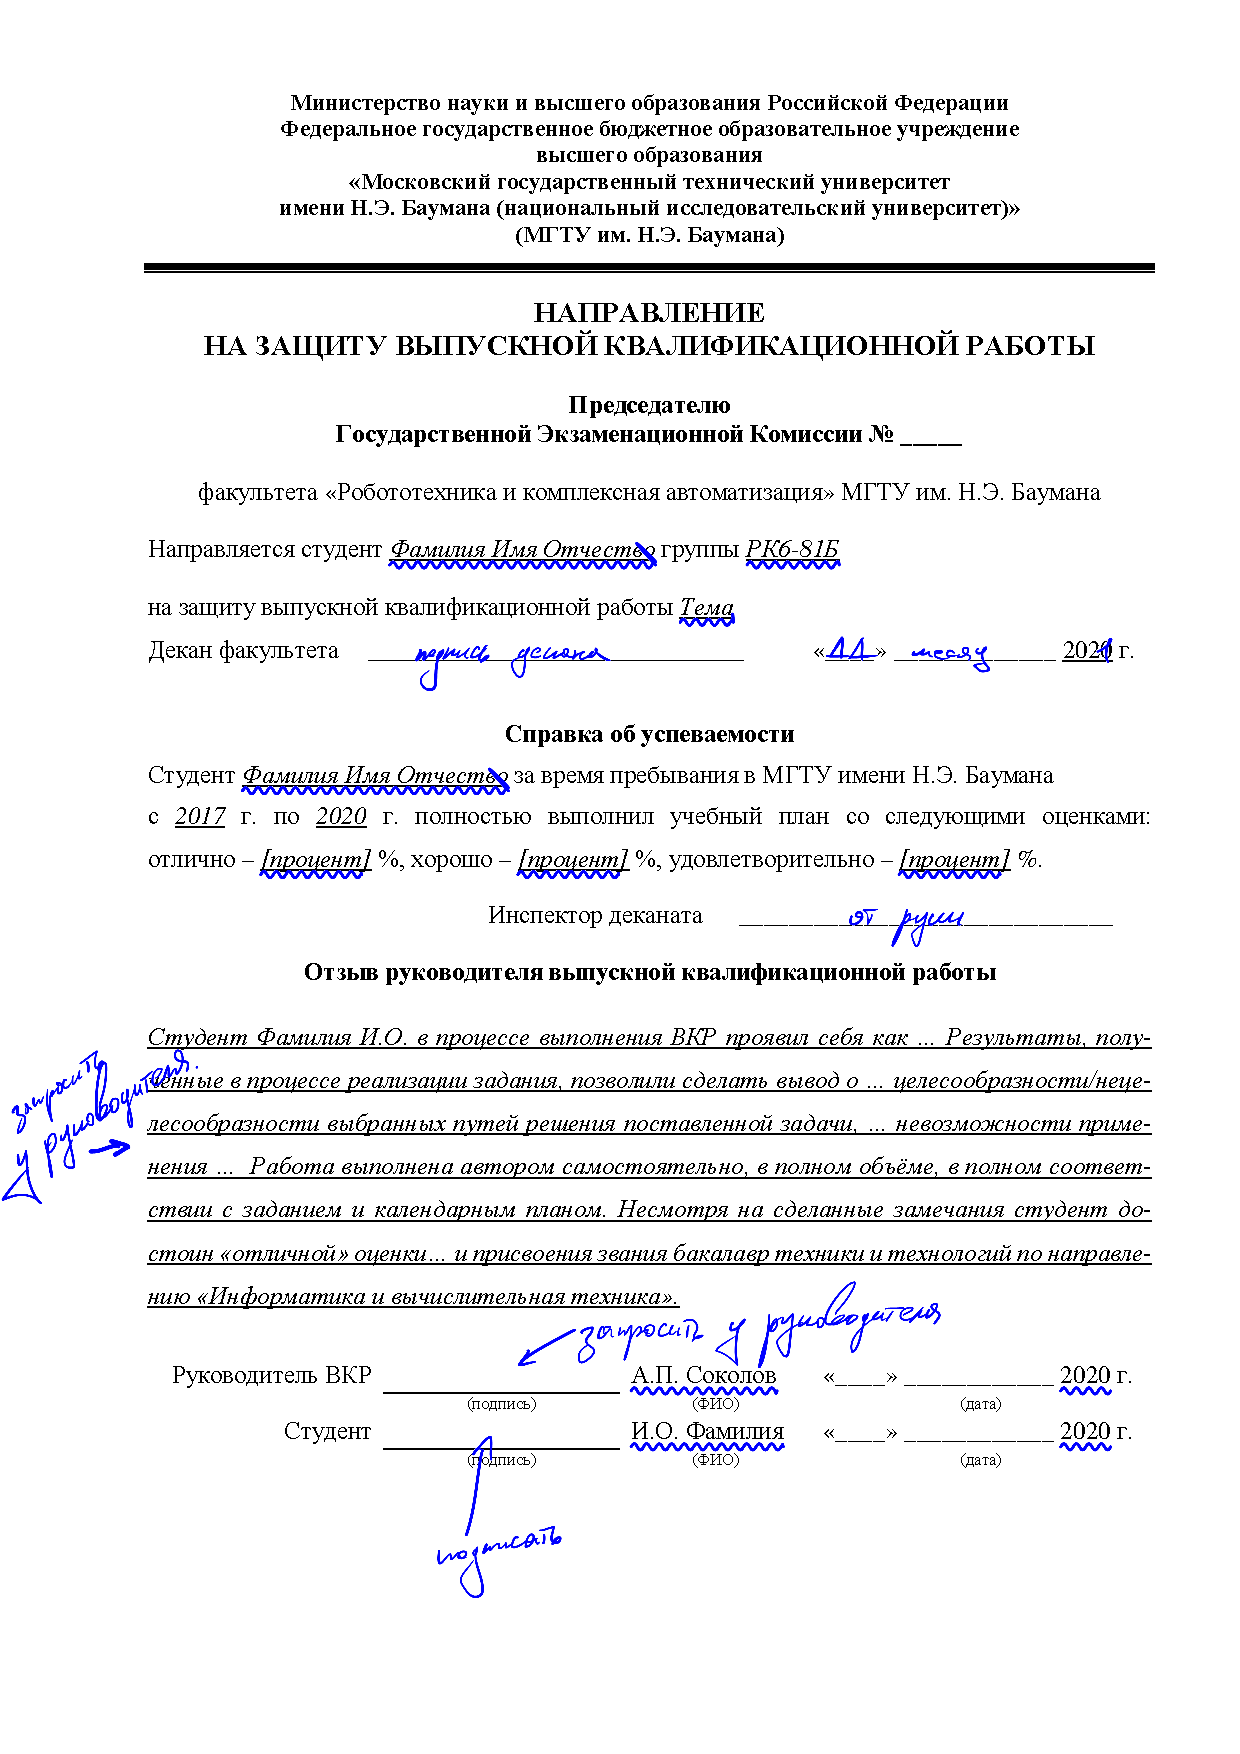
\includepdf{doc-additional/cpxsln_vkr_20YY_ShortTitle_group_SurnameNF_referral_for_defense_signed.pdf}
}
%----------------------------------------------------------------

} 
%----------------------------------------------------------
% Реферат
%----------------------------------------------------------
\chapter*{РЕФЕРАТ}
%----------------------------------------------------------
\doctype\xspace: \total{page}~с., \total{cchapter}~глав, \total{ffigure}~рис., \total{ttable}~табл., \total{bibcnt}~источн.%, \textbf{apxchapters} прил.

\vspace{3mm}

%Ключевые слова:
% \MakeUppercase{\keywordsru}.

\Preface

\textbf{Тип работы}: \doctype.

\textbf{Тема работы}: \textit{<<\Title>>}.

\textbf{Объект исследования}: \ObjectOfResearch.

% При оформлении согласно ГОСТ 7.32-2001 
%(все освещать следует в этом же порядке - разделы не обязательны)
%объект исследования или разработки
%цель работы
%метод или методологию проведения работы
%результаты работы
%основные конструктивные, технологические и технико-эксплуатационные характеристики
%степень внедрения
%рекомендации по внедрению или итоги внедрения результатов НИР
%область применения
%экономическую эффективновность или значимость
%прогнозные предположения о развитии объекта исследования.


%----------------------------------------------------------
% Сокращения и определения
\newpage
\pagestyle{fancy}
\printglossary[type=\acronymtype, title={СОКРАЩЕНИЯ}, nopostdot=false]
%\thispagestyle{plain}
%\printglossary[type=main, title={ОПРЕДЕЛЕНИЯ}, nopostdot=true]
%----------------------------------------------------------
% Содержание
% Глубина содержания должна быть не более, чем глава (chapter), раздел (section) и подраздел (subsection) 
\setcounter{tocdepth}{2}
% Добавление в оглавление сверху Стр.
%\makeatletter
%\addtocontents{toc}{\string\pagestyle{TOC}}
%\addtocontents{toc}{\string\thispagestyle{fancy}}
%\addtocontents{toc}{\hfill Стр.\par}
%\def\ps@TOC{%
    %\def\@oddhead{\hfill \thepage \hfill Стр.} % нечетные хедеры
    %\let\@oddfoot\@empty % нечетные футеры
    %\def\@evenhead{\hfill \thepage \hfill Стр.} % четные хедеры
    %\let\@evenfoot\@empty % четные футеры
%}
%\makeatother
%----------------------------------------------------------
\renewcommand{\contentsname}{\MakeUppercase{Содержание}}
\newpage
\tableofcontents
%----------------------------------------------------------
% Введение
{%
\def\thesection{В.\arabic{section}}
\def\thefigure{В.\arabic{figure}}
\def\thetable{В.\arabic{table}}
%----------------------------------------------------------
\chapter*{ВВЕДЕНИЕ}\label{chap.introduction}
\addcontentsline{toc}{chapter}{ВВЕДЕНИЕ}
% =========================================================================== %
% ----------------------------- ОСНОВНЫЕ ПУНКТЫ ----------------------------- %
% 1. Описание задач, в которых нужно всякое навороченное математическое ПО
% 2. Примеры наовороченного математического ПО
%   2.1. Почему просто математического ПО не всегда достаточно?
%   2.2. Упомянуть про задачи, у которых одна и та же постановка, но разные 
%         параметры
% 3. Примеры ПО, которое рассчитано на многократное решение задач, автоматизи-
%    рующее их решение (Scientific workflow, hallo?)
%   3.1. Использование графов при описании логики решения в системах научных
%        расчётов
%   3.2. Неудобства в описании данных
%   3.3. Визуальное программирование
% 4. Итог: нужно ПО, где есть какая-то абстракция над обрабатываемыми данными,
%    где они конкретизируются непосредственно в реализациях этапов алгоритма.
% 5. Enter GBSE and comsdk
%    5.1. А чем оно, собсна, так привлекательно?
%    5.2. Сказать про НОВЫХ пользователей (Р А С Ш И Р Я Е М О С Т Ь)
% 6. Сравнение GBSE и DFD
% =========================================================================== %
Современные научно-технические исследования зачастую включают в себя задачи, при решении которых требуется большое количество вычислений, для которых задействуются большие вычислительные мощности. К таким задачам относятся, например, задачи анализа, определения характеристик материалов или технических объектов, моделирования сложных динамических процессов. Как правило, для решения подобных задач применяется или разрабатывается специализированное программное обеспечение (далее -- \glsxtrshort{ПО}).

Среди прочих применяются программные продукты, предоставляющие пользователю формальный язык описания математических выражений и его интерпретатор, выполняющий необходимые вычисления на машине пользователя. К таким системам относятся, например, Mathcad. Также стоит отметить системы специализирующиеся на символьной алгебре, такие, как Maple\cite{CharMaple1983} и Wolfram Mathematica. В настоящее время данные программные комплексы поддерживают решение задач из различных областей математики, включающих в себя теорию графов, теорию множеств и~т.д, предоставляют инструменты визуализации и анализа результатов. Все они позволяют выполнять математическое моделирование, в том числе, сложных технических объектов. При всех их преимуществах необходимость формулировать математические постановки решаемых задач (т.е.~формировать математические модели, составлять системы уравнений и~т.д.) остаётся за пользователем. Зачастую требуется решать множество задач с схожей постановкой, но с различными входными параметрами. Такая необходимость, например, возникает при решении задач оптимизации, где критерием является некоторая характеристика, получаемая в результате решения задачи анализа. Следовательно, целесообразны автоматизированные средства решения типовых задач анализа и моделирования.

Данные средства относятся к специализированному \glsxtrshort{ПО}, а потому при их разработке требуются глубокие познания в предметной области. Кроме того, важно, чтобы создаваемая кодовая база была рассчитана на дальнейшую поддержку, что предъявляет соответствующие требования к структуре исходного кода и документации. Таким образом целесообразно применение некоторых средств, позволяющих организовать разработку программного обеспечения для решения задач моделирования и анализа и повысить его поддерживаемость.

В наши дни популярность приобретает применение т.н. научных систем управления потоком задач (англ.~scientific workflow systems). Они предоставляют средства организации этапов решения вычислительной задачи и управления вычислительными ресурсами. Процесс работы с подобными системами состоит из 4 основных этапов:
\begin{enumerate}[1)]
  \item составление описания операций обработки данных и зависимостей между ними;
  \item распределение процессов обработки данных по вычислительным ресурсам;
  \item выполнение обработки данных;
  \item сбор и анализ результатов и статистики~\cite{DeelmanWorkflow2009}.
\end{enumerate}

Примерами подобных систем могут служить Pegasus\cite{DeelmanPegasus2016}, Kepler\cite{AltintasKepler2004} и pSeven\cite{NazarenkoDFM2015}. Помимо инструментов загрузки пользовательских реализаций этапов решения задачи они, как правило, представляют библиотеку типовых действий и преобразований, таких, как считывание данных и их сохранение в файлы одного из поддерживаемых форматов, операции со строками, работы с базами данных, и~т.д. Кроме того, некоторые из них имеют средства интеграции с другими системами моделирования и анализа, что позволяет задействововать их при расчётах. На рисунке~\ref{fig:intro.keplerScreenshot} изображён пример описания некоторого процесса в системе Kepler.
\begin{figure}[!ht]
  \centering
  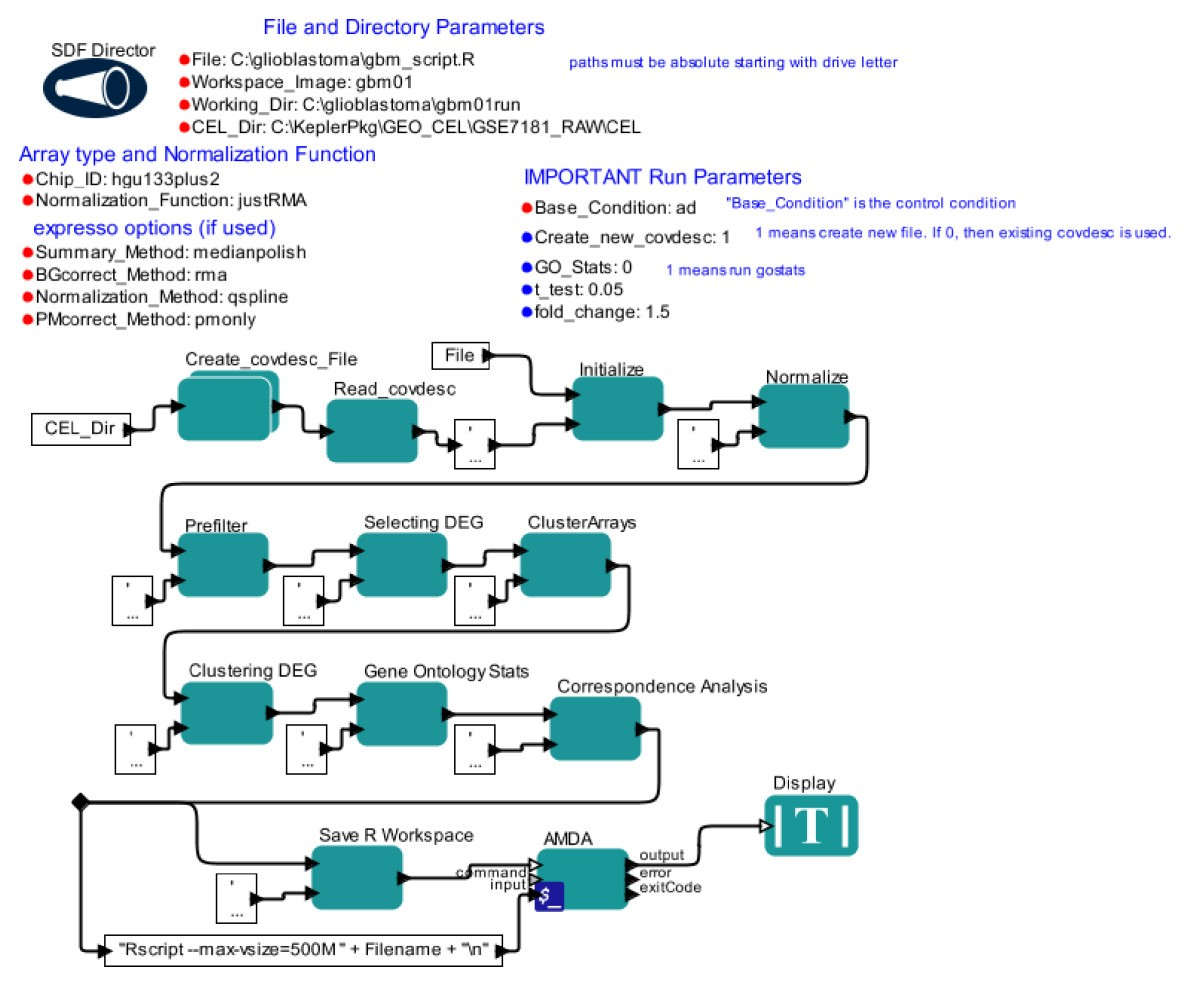
\includegraphics[height=0.35\textheight]{figures/screenshot.KeplerWorkflow.jpg}
  \caption{Описание процесса обработки данных в системе Kepler}
  \label{fig:intro.keplerScreenshot}
\end{figure}

Кроме того, для облегчения процесса разработки трудоёмкого ПО существуют т.н. платформы малокодовой разработки (англ.~low-code development platforms, \glsxtrshort{LCPD})\cite{DiRuscio2022}. В них, подобно системам управления потоком задач, логика разрабатываемого программного продукта описывается при помощи некоторого формального языка или с использованием графического редактора. От системы к системе подход к описаниям варьируется. Может применяться структурный подход, описывающий шаги алгоритма, или предметно-ориентированный, при котором описываются взаимодействующие сущности. Некоторые системы позволяют по созданному описанию генерировать готовые компоненты будущего программного продукта. Так платформа Codebots реализует предметно-ориентированный подход и по составленным UML-диаграммам взаимодействующих сущностей позволяет генерировать \glsxtrshort{API}, \glsxtrshort{JSON}-схемы данных и документацию\cite{DiRuscio2022}. Тем не менее, при реализации сложных вычислительных методов целесообразнее использовать структурный подход.

Одной из ключевых особенностей описанных технологических решений является выделение операций обработки данных в отдельные программные модули (функции, подпрограммы, скрипты). Как правило, при создании описаний алгоритмов в них используется следующий подход. Поскольку известно, что выходные данные одного программного модуля могут являться входными для одного или нескольких других модулей, можно сказать, что между ними формируются зависимости по входным и выходным данным. Тогда возможно составить такой ориентированный граф, описывающий общую логику алгоритма, в котором узлами являются операции обработки данных, а рёбрами -- пути данных. Такой подход получил название ``диаграммы потоков данных'' (англ.~Dataflow Diagram, \glsxtrshort{DFD}). На рисунке~\ref{fig:exampleDataflow} приведён пример такого ориентированного графа, описывающего процесс вычисления среднего арифметического и среднего геометрического двух массивов вещественных чисел.
\begin{figure}
  \centering
  \includegraphics[width=\textwidth]{figures/example.dataflow.png}
  \caption{Пример диаграммы потоков данных}
  \label{fig:exampleDataflow}
\end{figure}

При известных входных и выходных данных каждого модуля они могут создаваться независимо друг от друга\cite{DanilovPar2011}. Возникает возможность распределения задач создания отдельных программных модулей между разработчиками. Таким образом, уменьшается объём работы по написанию исходных кодов, приходящийся на одного исследователя. Это в свою очередь облегчает отладку и написание документации, что положительно сказывается на общем качестве реализуемого ПО.

В приведённом выше подходе существует необходимость явно описывать входные и выходные данные каждого процесса обработки. При этом на начальных этапах проектирования не всегда данные требуемые данные могут быть полность определены в силу недостатка представлений о программной реализации тех или иных этапов. Таким образом, в некоторых случаях может быть целесообразен такой подход к построению описания логики реализуемого решения, что в нём не указываются конкретные обрабатываемые данные. Последовательность выполнения отдельных этапов в таком случае должна задаваться явно. В предпринимательстве и управлении проектами подобный подход широко распространён и реализован в сетевых графиках. Сетевой график представляет собой ориентированный граф, в котором вершины -- это события или состояния проекта, а рёбра -- это работы. В работе~\cite{SokolovPershin2018} рассматривается применение идеи переходов между состояниями при описании логики вычислительных алгоритмов. Описанный подход получил название graph-based software engineering (\glsxtrshort{GBSE}). Кроме того в указанной работе описана реализация GBSE в библиотеке comsdk для языка C++.

Был проведён сравнительный анализ программного каркаса comsdk с аналогичным программным комплексом, в котором реализованы диаграммы потоков данных. В качестве такой реализации был рассмотрен программный комплекс pSeven, разработанный отечественной компанией DATADVANCE. Он направлен в первую очередь на решение конструкторских, оптимизационных задач и, помимо этого, задач анализа данных, что в первом приближении делает его аналогом comsdk по предметному назначению.

В терминах \textsf{pSeven}: графовое описание процесса решения задачи называется \textit{расчетной схемой} (англ.~workflow); вершинам графового описания поставлены в соответствие процессы обработки данных (используется термин \textit{блоки}), а рёбра определяют \textit{связи} между блоками и направления передачи данных между процессами~\cite{NazarenkoDFM2015}. При работе с pSeven используются следующие понятия:
\begin{itemize}
  \item \textsf{расчётная схема} -- формальное описание процесса решения некоторой задачи в виде ориентированного графа;
  \item \textsf{блок} -- программный контейнер для некоторого процесса обработки данных, входные и выходные данные для которого задаются через порты (см.~ниже);
  \item \textsf{порт} -- переменная конкретного\footnote{Динамическая типизация не поддерживается.} типа, определённая в блоке и имеющая уникальное имя в его пределах;
  \item \textsf{связь} -- направленное соединение типа ``один к одному'' между выходным и входным портами разных блоков.
\end{itemize}

С учётом данных понятий можно описать используемую методологию диаграмм потоков данных следующим образом. Расчётная схема содержит в себе набор процессов обработки данных (блоков), каждый из которых имеет (возможно, пустой) набор именованных входов и выходов (портов). Данные передаются через связи. Для избежания т.н. гонок данных (англ.~data races) множественные связи с одним и тем же входным портом не поддерживаются. Для начала выполнения каждому блоку требуются данные на всех входных портах. Все данные на выходных портах формируются по завершении исполнения блока~\cite{NazarenkoDFM2015}.

Сравнение реализаций двух подходов проводилось по следующим критериям:
\begin{itemize}
  \item особенности реализуемого подхода,
  \item особенности программной реализации,
  \item особенности взаимодействия пользователя с реализованной системой.
\end{itemize}
С учётом этого были выделены конкретные признаки для сравнения:
\begin{itemize}
  \item предметное назначение,
  \item значение вершины графа, описывающего алгоритм,
  \item значение ребра графа, описывающего алгоритм,
  \item топология графа, описывающего решение,
  \item поддержка иерархических графовых описаний, когда одно графовое описание является частью (ребром или вершиной) другого
  \item принцип передачи данных между отдельными этапами описываемого алгоритма,
  \item необходимость указывать входные и выходные данные каждого шага алгоритма
  \item язык программной реализации,
  \item файловый формат графовых описаний,
  \item файловая структура проекта реализуемого алгоритма,
  \item поддерживаемые типы данных,
  \item принцип ввода входных данных для алгоритма и его параметров,
  \item принцип вывода результатов работы алгоритма,
  \item поддержка параллельного выполнения незавимых шагов алгоритма,
  \item поддержка распределённого выполнения отдельных этапов алгоритма на вычислительном кластере,
  \item наличие графического редактора графовых описаний
  \item средства визуализации результатов работы алгоритма,
  \item поддержка алгоритмов, требующих принятие решения от пользователя,
  \item возможность дополнения набора входных данных во время работы алгоритма.
\end{itemize}

Результаты проведённого сравнения представлены в таблице \ref{rndhpcblo.0209}.

\begin{landscape}
  \begin{longtable}{|c|p{0.3\textwidth}|p{0.55\textwidth}|p{0.55\textwidth}|}
    \caption{Сравнительная таблица}\label{rndhpcblo.0209}                                                                                                                                                                                                                                                                                                                                                                                                                                                                                                                                                                                                                                                                                                                                                                                                                                                                                                                                                                                                           \\
    \hline
    \textbf{№} & \textbf{Признак}                                                                           & \textbf{pSeven}                                                                                                                                                                                                                                                                                                                                                                                                                                                                                                                                                                                                                                                   & \textbf{comsdk}                                                                                                                                                                                                                                                                   \\
    \hline
    1          & Предметное назначение                                                                      & Задачи оптимизации, анализ данных                                                                                                                                                                                                                                                                                                                                                                                                                                                                                                                                                                                                                                 & Задачи автоматизированного проектирования, алгоритмизация сложных вычислительных методов, анализ данных                                                                                                                                                                           \\
    \hline
    2          & Значение вершины графа, описывающего алгоритм                                              & Блок (процесс обработки данных)                                                                                                                                                                                                                                                                                                                                                                                                                                                                                                                                                                                                                                   & состояние данных                                                                                                                                                                                                                                                                  \\
    \hline
    3          & Значение ребра графа, описывающего алгоритм                                                & Связь (направление передачи данных)                                                                                                                                                                                                                                                                                                                                                                                                                                                                                                                                                                                                                               & переход меду состояниями с указанием функций, осуществляющих переход                                                                                                                                                                                                              \\
    \hline
    4          & Топология графа, описывающего решение                                                      & По умолчанию поддерживаются только ациклические графы. Поддерживаемая топология расширяется засчёт специальных управляющих блоков, которые отслеживают выполнение условий: для условного ветвления используется блок "Условие" (англ. condition), который перенаправляет данные на один из выходных портов в зависимости от выполнения описанного условия (подробнее см. \cite{pSevenDocsConditons2022}); Для реализации циклов в общем случае используются блоки "Цикл" (англ. loop)\cite{pSevenDocsWorkflow2021}, но для некоторых задач существуют специализированные блоки, организующие логику работы цикла (например, блок "Оптимизатор" (англ.~optimizer)) & Любая                                                                                                                                                                                                                                                                             \\
    \hline
    5          & Поддержка иерархических графовых описаний                                                  & \multicolumn{2}{c|}{Присутствует}                                                                                                                                                                                                                                                                                                                                                                                                                                                                                                                                                                                                                                                                                                                                                                                                                                                                                                                     \\
    \hline
    6          & Принцип передачи данных между отдельными этапами описываемого алгоритма                    & Данные между узлами передаются согласно определйнным связям, которые на уровне выполнения создают пространство в памяти для ввода и вывода данных для выполняемых в раздельных процессах блоков. Транзитная передача данных, которые не изменяются в данном блоке, на выход невозможна.                                                                                                                                                                                                                                                                                                                                                                           & Поскольку узлами графа являются состояния данных, существует возможность задействовать в расчётах только часть данных, оставляя их другую часть неизменной. Фактической передачи данных не производится.                                                                          \\
    \hline
    7          & Необходимость указывать входные и выходные данные каждого шага алгоритма                   & Присутствует                                                                                                                                                                                                                                                                                                                                                                                                                                                                                                                                                                                                                                                      & Отсутствует                                                                                                                                                                                                                                                                       \\
    \hline
    8          & Язык программной реализации                                                                & \multicolumn{2}{c|}{С++, Python}                                                                                                                                                                                                                                                                                                                                                                                                                                                                                                                                                                                                                                                                                                                                                                                                                                                                                                                      \\
    \hline
    9          & Файловый формат графовых описаний                                                          & Расчетная схема (в форме орграфа) сохраняется в двоичный файле закрытого формата с расширением \textsf{.p7wf}.                                                                                                                                                                                                                                                                                                                                                                                                                                                                                                                                                    & Графовая модель (определяет алгоритм проведения комплексных вычислений в форме орграфа) сохраняется в текстовом файле открытого формата, подготовленного на языке \gls{aDOT}\cite{SokolovADOT2020}, являющегося ``сужением'' (частным случаем) известного формата DOT (Graphviz). \\
    \hline
    10         & Файловая структура проекта реализуемого алгоритма                                          & Проект состоит из непосредственно файла проекта, в котором хранятся ссылки на созданные расчётные схемы и локальную базу данных, сами расчётные схемы, файлы с их входными данными, файлы отчётов, где сохраняются выходные данные последних расчётов и результаты их анализа.                                                                                                                                                                                                                                                                                                                                                                                    & Проект состоит из \textsf{.aDOT} файла с описанием графа, \textsf{.aINI}-файлов с описанием форматов входных данных, библиотек функций-обработчиков, функций-предикатов и функций-селекторов, файлов, куда записываются выходные данные.                                          \\
    \hline
    11         & Поддерживаемые типы данных                                                                 & Целые числа, числа с плавающей точкой, строки, логические переменные, логические, целочисленные и вещественные векторы и матрицы                                                                                                                                                                                                                                                                                                                                                                                                                                                                                                                                  & Целые и вещественные числа, строки, целочисленные и вещественные векторы                                                                                                                                                                                                          \\
    \hline
    12         & Принцип ввода входных данных для алгоритма и его параметров                                & Входные данные должны быть указаны при настройках внешних входных портов расчётной схемы.                                                                                                                                                                                                                                                                                                                                                                                                                                                                                                                                                                         & Входные данные хранятся в файле в формате \gls{aINI}\cite{SokAINI}, откуда считываются при запуске обхода графа~\cite{SokolovPershin2017}.                                                                                                                                        \\
    \hline
    13         & Принцип вывода результатов работы алгоритма                                                & Данные с выходных портов схемы сохраняются в локальной базе данных. Для их записи в файлы для обработки/анализа вне pSeven необходимо воспользоваться специально предназначенными для этого блоками.                                                                                                                                                                                                                                                                                                                                                                                                                                                              & Для записи выходных/промежуточных данных в файлы или базы данных необходимо добавить соответствующие функции-обработчики. Формат выходных данных не регламентирован.                                                                                                              \\
    \hline
    14         & Поддержка параллельного выполнения независимых шагов алгоритма                             & Присутствует. Блоки, входящие в состав различных ветвлений схемы могут быть выполнены параллельно, поскольку они не зависят друг от друга по используемым данным.                                                                                                                                                                                                                                                                                                                                                                                                                                                                                                 & Присутствует. Существует возможность обойти различные ветвления графа одновременно.                                                                                                                                                                                               \\
    \hline
    15         & Поддержка распределённого выполнения отдельных этапов алгоритма на вычислительном кластере & Присутствует                                                                                                                                                                                                                                                                                                                                                                                                                                                                                                                                                                                                                                                      & В текущей версии отсутствует                                                                                                                                                                                                                                                      \\
    \hline
    16         & Наличие графического редактора графовых описаний                                           & Да                                                                                                                                                                                                                                                                                                                                                                                                                                                                                                                                                                                                                                                                & Да\footnote{В виде отдельного веб-приложения}                                                                                                                                                                                                                                     \\
    \hline
    17         & Средства визуализации результатов работы алгоритма                                         & Реализованы как часть системы формирования отчётов (см. выше)                                                                                                                                                                                                                                                                                                                                                                                                                                                                                                                                                                                                     & В текущей версии отсутствуют                                                                                                                                                                                                                                                      \\
    \hline
    18         & Поддержка алгоритмов, требующих принятие решения от пользователя                           & По умолчанию отсутвует. Требуется реализация дополнительных скриптов на языке Python, отвечающих за взаимодействие с пользователем                                                                                                                                                                                                                                                                                                                                                                                                                                                                                                                                & Частично присутствует засчёт средства генерации форм ввода\cite{SokolovPershin2017}                                                                                                                                                                                               \\
    \hline
    19         & Возможность дополнения набора входных данных во время работы алгоритма                     & Отсутствует                                                                                                                                                                                                                                                                                                                                                                                                                                                                                                                                                                                                                                                       & Частично реализована при помощи функций-обработчиков специального типа, создающих формы ввода                                                                                                                                                                                     \\
    \hline
  \end{longtable}
\end{landscape}

Таким образом, на данный момент comsdk обладает сравнительно меньшим числом функциональных возможностей, чем современные научные системы управления потоком задач, подобные pSeven, но предоставляет потенциально больше средств для взаимодействия реализуемых алгоритмов с пользователем. В условиях существующей на сегодняшней день потребности в отечественном программном обеспечении для реализации сложных численных методов, актуально развитие данного программного каркаса.
}
%----------------------------------------------------------
\mainmatter %% это включает нумерацию глав и секций в документе ниже
%----------------------------------------------------------
%=============================================================
%----------------------------------------------------------
\chapter{Постановка задачи}
\label{ch:task}
%----------------------------------------------------------


\section{Концептуальная постановка задачи}
\label{sec:abstract_task}

Объект разработки: система типов

Цель: реализовать систему вывода и проверки типов

Задачи:
\begin{enumerate}[1)]
    \item спроектировать представления AST в компиляторе,
    \item реализовать анализатор областей видимости,
    \item написать алгоритм для вывода типов.
\end{enumerate}

%----------------------------------------------------------


\section{Математическая постановка задачи}
\label{sec:math_task}

\todo{Поставить задачу}
%----------------------------------------------------------
%----------------------------------------------------------
\chapter{Аналитический обзор}\label{chap2_review}
%----------------------------------------------------------
Одними из первых рассмотренных были форматы для хранения научных данных HDF4 и HDF5~\cite{HDFOffCite}. Данные бинарные форматы позволяют хранить большие объёмы гетерогенной информации и поддерживают иерархическое представление данных. В нём используется понятие набора данных (англ. dataset), которые объединяются в группы (англ. group). Кроме того, формат HDF5 считается <<самодокументирующимся>>, поскольку каждый его элемент -- набор данных или их группа -- имеет возможность хранить метаданные, служащие для описания содержимого элемента. Существует официальный API данного формата для языка С++ с открытым исходным кодом. Одним из гланвых недостатков HDF5 является необходимость дополнительного ПО для просмотра и редактирования данных в этом формате, поскольку он является бинарным.

Альтернативой бинарным форматам описания данных являются текстовые. Среди них были рассмотрены форматы XML (Extensible Markup Language) и JSON (Javascript Object Notation). Главным преимуществом формата XML является его ориентированность на древовидные структуры данных и лёгкость лексико-синтаксического разбора файлов этого формата. Среди недостатков стоит выделить потребность в сравнительно большом количестве вспомогательных синтаксических конструкций, необходимых для структурирования (тегов, атрибутов). Они затрудняют восприятие чистых данных и увеличивают итоговый объём файла.

Формат JSON, так же, как и XML рассчитан на иерархические структуры данных, но является не столь синтаксически нагруженным, что облегчает восприятие информации человеком~\cite{JSONvsXML}. Кроме того, крайне важным преимуществом JSON является его поддержка по-умолчанию средствами языкы программирования Javascript, который используется при разработке веб-приложений. При этом JSON также обладает рядом недостатков. Среди них сниженная, по сравнению с XML надёжность, отсутствие встроенных средств валидации и отсутствие поддержки пространств имён, что снижает его расширяемость.

На основании проведённого анализа преимуществ и недостатков выбор был сделан в пользу формата JSON. Ключевыми факторами для этого стали лёгкость восприятия информации в этом формате и нативная поддержка этого формата языком Javascript.

%----------------------------------------------------------


%----------------------------------------------------------
%----------------------------------------------------------
\chapter{Программная реализация}
\label{ch:chap3_soft_architecture}
%----------------------------------------------------------


Прототип компилятора для языка Kodept разрабатывается с использованием языка программирования Rust.
Этот язык предлагает надежный концепт управления памятью, не имея при этом сборщика мусора~\cite{RustMemory}.
Кроме того, он соперничает по скорости с C и C++ и применяется в довольно широком спектре приложений.
Основные преимущества выбора этого языка:
\begin{itemize}
    \item Rust работает быстрее за счёт использования мощных оптимизаторов, а так же применяет более строгие требования к разработке в целом,
    \item он предоставляет больше гарантий разработчику, как посредством его системы типов, так и другими средствами, например, borrow checker~\cite{RustBchk},
    \item система сборки создает нативный файл программы~--- его можно запустить, не имея на машине специальных сред выполнения.
\end{itemize}

Важным внутренним элементом программы является абстрактное синтаксическое дерево (англ. abstract syntax tree, AST).
Оно в абстрактном виде представляет структуру исходного кода и используется во многих частях компилятора.
Вершинами дерева является набор объектов, описывающих тот или иной синтаксический элемент.
Для удобства обобщенная вершина этого дерева будет называться \lstinline{ASTNode}.

\section{Варианты использования прототипа компилятора}
\label{sec:usage}

Были составлены варианты использования прототипа компилятора с точки зрения как пользователя программы, так и разработчика проекта~\figref{fig:usage}.
Разработчик компилятора выделен как отдельное действующее лицо, так как ему необходим доступ к расширенной информации о работе процесса компиляции.
Важно понимать, что компилятор всё ещё находится в разработке, поэтому в будущем будет добавлено больше вариантов использования.
Реализация существующих вариантов выполнена в виде набора команд и флагов для интерфейса командной строки.

\begin{figure}[H]
    \centering
    \input{figures/.generated/usage}
    \caption{UML-диаграмма вариантов использования прототипа компилятора языка Kodept}
    \label{fig:usage}
\end{figure}

Рассмотрим варианты использования подробнее.
Пользователь программы взаимодействует с ней посредством интерфейса командной строки (англ. command line interface, CLI).
При этом на выбор ему доступны две команды, отражающие соответсвующий вариант использования: для обработки файла~--- команда \lstinline{run}, для сохранения структуры AST~--- команда \lstinline{graph}.
Приведём пример использования CLI:
\[
    \underbracket{\text{\lstinline{kodept}}}_{\text{имя исполняемого файла}}~
    \underbracket{\text{\lstinline{graph}}}_{\text{команда}}~
    \underbracket{\text{\lstinline{-d -o output}}}_{\text{опции запуска}}~
    \underbracket{\text{\lstinline{examples/church.kd}}}_{\text{путь до исходного файла}}
\]

В результате работы команды \lstinline{graph} будет получен файл, содержащий представление AST на языке \lstinline{dot}~\cite{Dot}.
Примером отрисовки такого файла является рисунок~\ref{fig:ast_dot}.
В процессе выполнения команды компилятор выполняет первые два шага~--- синтаксический и лексический анализы, а затем строит абстрактное синтаксическое дерево.
Эта команда подразумевается в отладочных целях.

Другая команда~---~\lstinline{run} является более комплексной, по сравнению с предыдущей.
В результате её выполнения будут выведены все собранные \textit{диагностики}.
Во время работы команда выполняет лексический, синтаксический и семантический анализы, в том числе и вывод типов.
В будущем подразумевается, что она будет проводить полный цикл компиляции~\figref{fig:pipeline}.
Кроме команд, используются опции компиляции, полный список которых приведён в таблице~\ref{tab:flags}.

\begin{table}[H]
    \centering
    \caption{Опции командной строки, используемые в компиляторе языка Kodept}
    \label{tab:flags}
    \begin{tabular}{|p{25mm}|p{0.25\textwidth}|p{0.5\textwidth}|}
        \hline
        \textbf{Короткое название} & \textbf{Полное название}       & \textbf{Описание}                                  \\\hline
        \texttt{-d}                & \texttt{--debug}               & Включение отладочной печати                        \\\hline
        \texttt{-v}                & \texttt{--verbose}             & Включение подробной печати                         \\\hline
        \texttt{-s}                & \texttt{--severity}            & Установка уровня логирования по-умолчанию          \\\hline
        \texttt{-o}                & \texttt{--out}                 & Путь для записи выходных данных                    \\\hline
        & \texttt{--style}               & Стиль отображения диагностик                       \\\hline
        & \texttt{--tab-width}           & Добавление отступов                                \\\hline
        \texttt{-c}                & \texttt{--color}               & Использование цветной печати                       \\\hline
        & \texttt{--disable-diagnostics} & Отключить вывод диагностик                         \\\hline
        & \texttt{--stdin}               & Чтение входных данных из потока стандартного ввода \\\hline
        \texttt{-e}                & \texttt{--extension}           & Использовать указанное расширение для файлов       \\\hline
        \texttt{-V}                & \texttt{--version}             & Получить версию программы                          \\\hline
    \end{tabular}
\end{table}

Диагностика (диагностическое сообщение)~---сообщение компилятора, выводимое в стандартный поток ошибок.
Она необходима для указания проблемы, ошибки или другой вспомогательной информации об исходном коде.
Диагностики формируются в нескольких местах при выполнении программы.
Например, после синтаксического анализа, все встреченные ошибки синтаксиса трансформируются в диагностики.
Ниже приведен пример диагностики для некоторой функции \lstinline{test} на языке Kodept.

\begin{verbatim}
    note[TC001]: `test` inferred to: Floating -> Floating
  ┌─ examples/test.kd:5:9
5 │     fun test(m) {
  │         ^^^^
\end{verbatim}

Формат диагностики может меняться в зависимости от опций компиляции, но упрощённо выглядит следующим образом:

\begin{align*}
    &\underbracket{\text{\lstinline{bug}}}_{\mathclap{\text{важность}}}
    \underbracket{\text{\lstinline{[TC002]:}}}_{\text{код}}~
    \underbracket{\text{\lstinline{Unimplemented}}}_{\text{основное описание}}\\
    &\underset{\text{место в исходном файле}}{\text{\lstinline{examples/test.kd:9:10}}}\\
    &\text{\lstinline{// code...}}
\end{align*}
\begin{eqrem}
    & важность~--- уровень важности диагностики, может быть \texttt{note}, \texttt{info}, \texttt{error} и пр., \\
    & код~--- пятибуквенный номер, идентифицирующий диагностику.
\end{eqrem}


\section{Архитектура прототипа компилятора}
\label{sec:arch}

В структуре программы почти любого компилятора можно выделить 3 основные части~\cite{CraftingInterpreters}:
frontend, отвечающий за обработку исходного вода, backend, ответственный за работу с внутренним представлением программы и middle-end, выступающий в роли связующего звена.
Следует отметить, что, хоть названия частей и похожи, они имеют мало общего с одноимёнными названиями из сферы веб-разработки.
На рисунке~\ref{fig:pipeline} также отмечены внутренние элементы каждой из частей, а стрелки показывают данные, передаваемые от стадии к стадии.
Результатом компиляции является объектный модуль (файл), в котором содержатся набор символов, отладочная информация, константные данные и др.
Символы в объектном файле представляют собой именованные объекты, позволяющие идентифицировать функции, переменные, типы данных.

\begin{figure}[H]
    \centering
    \input{figures/.generated/pipeline}
    \caption{Схема состояний работы компилятора}
    \label{fig:pipeline}
\end{figure}

Реализация системы типов, описанной в разделе~\ref{sec:hindley-milner}, в языке Kodept является одной из основных задач этой работы.
Поэтому будет подробно рассмотрен семантический анализатор, включающий механизм вывода типов.
Процесс разработки frontend части компилятора был завершён до этой работы и подробно раскрываться не будет.

На рисунке~\ref{fig:semantic_classes} дано более подробное описание семантического анализатора.
При этом сплошная стрелка отображает ассоциацию между объектами, а штриховая~--- зависимость в направлении от зависимого к главному.
С помощью записи \lstinline{0..*} у объекта указывается, что таких объектов может быть от 0 и больше.

\begin{figure}[h]
    \centering
    \input{figures/.generated/arch}
    \caption{UML-диаграмма классов, связанных с семантическим анализатором}
    \label{fig:semantic_classes}
\end{figure}


\section{Разбиение на модули}
\label{sec:modules}

Работать с большими проектами в разы удобнее и эффективнее при грамотном разбиении на модули.
В экосистеме языка Rust такие модули именуются крейтами (англ. crates).
На рисунке~\ref{fig:modules} представлено разбиение на модули проекта Kodept.
При этом стрелки указывают на зависимость одного модуля от другого.

\begin{figure}[H]
    \centering
    \input{figures/.generated/modules}
    \caption{Диаграмма иерархии модулей в исходном коде компилятора Kodept}
    \label{fig:modules}
\end{figure}

В рамках этой работы внимание будет сконцентрировано вокруг модулей \lstinline{kodept-ast}, \lstinline{kodept-interpret} и \lstinline{kodept-inference}, так как именно с помощью них решаются поставленные задачи.
Однако, дадим краткое описание остальных модулей:
\begin{itemize}
    \item \lstinline{kodept-core} отвечает за определение основных структур данных, необходимых в остальных частях приложения, в частности, в нем определена структура \textit{дерева разбора},
    \item \lstinline{kodept-parse} отвечает за лексический и синтаксический анализ, определяя набор синтаксических анализаторов (парсеров), которые генерируют дерево разбора,
    \item \lstinline{kodept-macros} нужен для работы с AST и создания диагностик,
    \item \lstinline{kodept} является корневым модулем и обеспечивает запуск стадий компилятора для входных файлов,
    \item \lstinline{slotgraph} содержит реализацию графа с использованием \textit{генеративной арены}.
\end{itemize}

Дерево разбора (англ. raw lexem tree, RLT)~---подробное синтаксическое дерево, включающее в себя полную информацию об исходном коде.
Необходимо для восстановления конкретной точки в программе при создании диагностики.
В процессе работы программы трансформируется в AST, где каждый узел RLT соответствует определенному узлу AST.

Генеративная арена~--- специальный вид контейнера для объектов в программировании, в котором для каждого объекта присваивается не только уникальный идентификатор, но и поколение.
Благодаря этому решается проблема утечек памяти: когда удаляется объект из обычной арены, то его место ничем не может быть занято, чтобы не нарушить идентификатор.
В то же время в генеративной арене место из-под удалённого объекта может быть переиспользовано с помощью изменения поколения.

В модуле \lstinline{kodept-ast} определена структура AST и принципы его хранения.
Рассмотрим некоторые технические решения, реализованные при проектировании этого модуля.


\section{Организация хранения абстрактного синтаксического дерева}
\label{sec:ast_structure}

Обычно абстрактное синтаксическое дерево реализовано в программе в виде вложенных друг в друга структур с данными, описывающими тот или иной синтаксис языка.
Например, внутреннее представление функции с набором именованных параметров реализовано композицией структур~\figref{fig:func_AST}.

\begin{figure}[H]
    \centering
    \input{figures/.generated/AST_func}
    \caption{Диаграмма классов, представляющих собой узел функции в AST}
    \label{fig:func_AST}
\end{figure}

Основным процессом при работе семантического анализа является обход абстрактного синтаксического дерева с целью применения различных алгоритмов.
Распространено использование так называемого шаблона посетитель (англ. visitor).
Это специальная структура данных, содержащая алгоритмы для обработки каждой вершины дерева.

У такого подхода есть несколько минусов:
\begin{inparaenum}[1)]
    \item обход совершается в рекурсивном стиле, а это значит, что компилятор не способен обрабатывать большие исходные программы,
    \item сложно поддерживать, так как необходимо изменить или добавить необходимые функции в код каждого посетителя при изменении вида AST,
\end{inparaenum}

В итоге был использован другой подход.
Вместо хранения всех структур <<вложенными>> друг в друга~\figref{fig:func_AST}, было решено применить <<графовый>> метод.
Суть его заключается в создании структуры-контейнера \lstinline{SyntaxTree}.
Все исходные структуры переписываются так, что из них убираются любые вложенные структуры, кроме базовых полей (имя и прочее).
Также добавляется специальное поле \lstinline{id}.
Диаграмма классов после преобразования представлена на рисунке~\ref{fig:func_AST_after}.

Такая композиция позволяет хранить все объекты AST в одном месте, линейно.
Кроме того, реализация обхода дерева перестаёт быть рекурсивной и является реализацией алгоритма обхода в глубину.
Для сохранения взаимосвязи между структурами, вводятся методы доступа.
На рисунке~\ref{fig:func_AST_after} таким методом будет \lstinline{parameters}.

\begin{figure}[H]
    \centering
    \input{figures/.generated/AST_func_after}
    \caption{Диаграмма классов после введённого преобразования}
    \label{fig:func_AST_after}
\end{figure}

Рассмотрим подробнее структуру AST на рисунке~\ref{fig:ast_dot}.
В вершинах дерева расположены имена соответствующих структур данных вместе с идентификатором.
Формат записи следующий: $\underset{\text{имя}}{\text{FileDecl}}~\text{[}\underset{\text{идентификатор}}{1}\text{v}\underset{\text{поколение}}{1}\text{]}$.
У всех вершин поколение равно единице, так дерево не модифицировалось.
На некоторых рёбрах дерева расположились теги~--- маркеры, с помощью которых можно различить одинаковые по имени, но разные по семантике структуры.
Например, обе вершины 11 и 12 являются ссылкой, но 11~--- телом, а 12~--- аргументом.


\section{Реализация алгоритма $\mathcal{W}_c$}
\label{sec:algorithm_W}

Реализация механизма вывода типов расположена в модуле \lstinline{kodept-inference}.
В нём также определены структуры для объектов, рассмотренных в разделе~\ref{sec:hindley-milner}.
Согласно рисунку~\ref{fig:modules}, этот модуль не зависит от остальных.
Достигается это тем, что часть AST конвертируется в эквивалентную структуру \lstinline{Language} из модуля \lstinline{kodept-inference}, представляющей собой терм~\eqref{eq:terms}.
Затем для неё выводится тип, используя методы этого же модуля.

В процессе конвертации используется информация из \textit{дерева областей видимости} (англ. scope tree) для правильного определения всех ссылок.
Под ссылкой будем понимать идентификатор, ссылающийся на другой элемент исходного кода.
Например, в листинге~\ref{lst:kodept}, ссылкой является переменная \lstinline{x} в записи \lstinline{f(g(x))}.

\subsection{Анализ областей видимости}
\label{subsec:scope_analysis}

Задачей этого анализа является разбиение AST на области видимости (англ. scopes), при котором строится так называемое дерево областей видимости.
Вершинами дерева является структура \lstinline{Scope}, представленная на рисунке~\ref{fig:scope_class}.
Принцип формирования дерева прост~--- обходится каждая вершина AST, если она является одной из вершин, которые образуют область видимости, то в дерево добавляется новый объект \lstinline{Scope}, содержащий идентификатор текущей вершины AST и её имя.
По мере обхода заполняются ассоциативные массивы для типов (\lstinline{types}) и переменных (\lstinline{variables}) текущей области видимости.
Благодаря им можно узнать, на что ссылалась та или иная ссылка с помощью методов \lstinline{get_var} и \lstinline{get_type}.

\begin{figure}
    \centering
    \input{figures/.generated/scope}
    \caption{UML-диаграмма класса, представляющего вершину в дереве областей видимости}
    \label{fig:scope_class}
\end{figure}

В список вершин, которые могут образовать область видимости, входят: \lstinline{ModDecl}, \lstinline{StructDecl}, \lstinline{EnumDecl}, \lstinline{AbstFnDecl}, \lstinline{BodyFnDecl}, \lstinline{FileDecl}, \lstinline{Exprs}, \lstinline{Lambda}, \lstinline{IfExpr}.

Рассмотрим образование дерева областей видимости~\figref{fig:scopes} на примере программы с листинга~\ref{lst:kodept}.
Рисунок~\ref{fig:ast_dot} является изображением абстрактного синтаксического дерева для этой программы.
В нём присутствует 7 вершин, образующих область видимости, однако в действительности областей 6, так как вершина с идентификатором 17 не имеет дочерних вершин.

\begin{figure}[H]
    \centering
    \input{figures/.generated/scopes}
    \caption{Дерево областей видимости; в каждом элементе дерева в квадратных скобках указывается идентификатор вершины, после~--- имя области видимости}
    \label{fig:scopes}
\end{figure}

\subsection{Преобразование AST в термы}
\label{subsec:ast_transformation}

Определенный в разделе~\ref{sec:inference_algo}, алгоритм вывода типов $\mathcal{W}_c$ не может работать со структурой абстрактного синтаксического дерева.
Для того чтобы проверить типы в программе, необходимо преобразовать AST в подходящую для алгоритма структуру.
При этом преобразуются не всё дерево, а лишь некоторая его часть.
Преобразование происходит с помощью функции \lstinline{convert(...)} по правилам, которые указаны ниже.
Будем использовать нотацию $\underline{e}$ для результата вызова функции \lstinline{convert(e)}.

Правило преобразования функции с телом \lstinline{BodyFnDecl [name, expr, parameters ]}, где \lstinline{parameters}~--- параметры функции, \lstinline{expr}~--- тело функции:

\begin{equation*}
%    \label{eq:conv_bfn}
    \begin{cases}
        \underline{expr} \text{ если параметров нет}, \\
        \lambda \underline{p1}. \lambda \underline{p2}. \cdots. \underline{expr},
    \end{cases}
\end{equation*}
\begin{eqrem}
    & \texttt{p1, p2} $\in$ \texttt{parameters}.
\end{eqrem}

Правило для преобразования применения \lstinline{Appl [ expr, parameters ]}:

\begin{equation*}
%    \label{eq:conv_appl}
    \begin{cases}
        \underline{expr} \text{ если параметров нет}, \\
        ((\underline{expr}(\underline{p1}))(\underline{p2}))\ldots,
    \end{cases}
\end{equation*}
\begin{eqrem}
    & \texttt{p1, p2} $\in$ \texttt{parameters}.
\end{eqrem}

Правило для преобразования набора выражений \lstinline{Exprs [ items ]}:

\begin{align*}
%    \label{eq:conv_exprs}
    \begin{cases}
    ()
        &\text{ если список \lstinline{items} пуст},\\
        \text{let } n = \underline{i1} \text{ in } (\underline{i2}) &\text{ если } \underline{i1} \ne \text{ let } x = e_1 \text{ in } e_2,\\
        \text{let } x = e_1 \text{ in } \underline{i2} &\text{иначе},
    \end{cases}
\end{align*}
\begin{eqrem}
    & \texttt{i1, i2} $\in$ \texttt{items},                                             \\
    & \texttt{n}~--- имя элемента \texttt{i1} (если есть, иначе~--- идентификатор вершины).
\end{eqrem}

Правило для преобразования объявления инициализированной переменной \lstinline{InitVar [ name, expr ]}:

\begin{equation*}
%    \label{eq:conv_initvar}
    \text{let } name = \underline{expr} \text{ in } name
\end{equation*}

Правило для преобразования условного выражения \lstinline{IfExpr [ condition, body, elifs, else ]}, где \lstinline{elifs}~--- список с элементами вида \lstinline{ElifExpr [ condition, body ]}, \lstinline{else} имеет вид \lstinline{ElseExpr [ body ]}:

\begin{equation*}
%    \label{eq:conv_if}
    \text{if } \underline{condition} \text{ then } \underline{body} \text{ otherwise } e_1,
\end{equation*}
\begin{eqrem}
    & $e_i = \text{ if } \underline{efi.condition} \text{ then } \underline{efi.body} \text{ otherwise } e_{i + 1}$, \\
    & $e_n = \underline{else}$,                                                                                      \\
    & \texttt{efi} $\in$ \texttt{elifs}.
\end{eqrem}

Правило для преобразования числовых литералов тривиально и представляет собой использование терма $\text{:num:}$.
Преобразование кортежа~--- преобразование каждого элемента внутри кортежа.
Правило для ссылки \lstinline{Ref [ name] }: $name$.

Правило для преобразования лямбда-функции \lstinline{Lambda [ binds, expr ]}, где \lstinline{binds}~--- список параметров лямбда-функции:

\begin{equation*}
%    \label{eq:conv_lambda}
    \begin{cases}
        \underline{expr} \text{ если параметров нет}, \\
        \lambda \underline{b1}. \lambda \underline{b2}. \cdots. \underline{expr},
    \end{cases}
\end{equation*}
\begin{eqrem}
    & \texttt{b1, b2} $\in$ \texttt{binds}.
\end{eqrem}

Вывод типов в программе проводится отдельно для каждого определения функции с телом.
При этом к структуре функции применяется функция \lstinline{convert} с последующим получением терма $e$.
Затем производится первый этап алгоритма $\mathcal{W}_c$~--- к терму $e$ применяются правила вывода в форме, определённой в разделе~\ref{subsec:inference_rules}.
Таким образом имеется набор предположений $\mathcal{A}$~\eqref{eq:assumption_set} и набор ограничений $\mathcal{C}$.
Для каждого элемента $x: \tau$ набора предположений рекурсивно запускается отдельный процесс преобразования узла AST, определяющего $x$, а результат процесса записывается в контекст $\Gamma$.
Благодаря этому второй этап алгоритма $\mathcal{W}_c$ имеет полностью определенный набор внешних определений $\Gamma$.

После решения ограничений с помощью алгоритма~\ref{eq:solve_algo}, будет получен тип $\tau$ для выражения $e$.
Этот тип обобщается~\eqref{eq:generalize} и выступает в качестве выведенного для рассматриваемой функции.

Рассмотрим работу функции \lstinline{convert} на примере листинга~\ref{lst:kodept}.
В нём содержится одна функция \lstinline{convert}, представляющая собой одно лямбда-выражение.
Последовательно применяя правила преобразования, можно получить следующий терм для этой функции: $\lambda f. \lambda g. \lambda x. f(g(x))$.

%----------------------------------------------------------

%----------------------------------------------------------
%----------------------------------------------------------
\chapter{Тестирование и отладка}
\label{ch:chap4_soft_testing}
%----------------------------------------------------------

При разработке приложения не обойтись без тестирования.
Оно помогает выявить различные ошибки и исправить их.
Популярным вариантом тестирования является модульное тестирование (unit тестирование).
Unit test - функция или набор функций, который проверяет корректность работы отдельного нетривиального куска программы.

В ходе разработки компилятора были написаны модульные тесты, они покрывают большое количество кода и успешно выполняются.
Для запуска можно использовать систему сборки Cargo.
Из папки с проектом следует запустить следующую команду:~\lstinline{cargo test --all-features --all --lib --no-fail-fast}.
Cargo соберет проект и последовательно запустит все модульные тесты.

\todo{Дописать}

%----------------------------------------------------------


%----------------------------------------------------------
%----------------------------------------------------------
\chapter{Вычислительный эксперимент}\label{chap5_comp_experiment}
%----------------------------------------------------------
\section{...}

В разделе следует представить описания каждого вычислительного эксперимента, включая указание особенностей их проведения, используемые программные средства, используемые исходные данные, принципы запуска с указанием ожидаемого и полученного результата.

Обязательно представление графических результатов в форме графиков, поверхностей.

Обязательность представления: раздел представляется в зависимости от постановки задачи.

Объём: объём не ограничен, но, как правило, не должен быть меньше 5-6 страниц.

%----------------------------------------------------------
%\section{...}

%----------------------------------------------------------


%----------------------------------------------------------
%----------------------------------------------------------
\chapter{Анализ результатов}\label{chap6_results_analysis}
%----------------------------------------------------------
\section{...}

В разделе следует представить анализ полученных результатов, вклюая указание перспектив развития созданных научно-технических решений.

Обязательность представления: раздел обязателен.

Объём: объём не ограничен, но, как правило, не должен быть меньше 2 страниц.

%----------------------------------------------------------
%\section{...}

%----------------------------------------------------------


%=============================================================

%----------------------------------------------------------
\backmatter %% Здесь заканчивается нумерованная часть документа и начинаются Заключение и Список использованных источников
%----------------------------------------------------------
%----------------------------------------------------------
\chapter*{ЗАКЛЮЧЕНИЕ}\label{chap_conclusion}
\addcontentsline{toc}{chapter}{ЗАКЛЮЧЕНИЕ}
%----------------------------------------------------------

В результате проведенной работы был реализован редактор графов, который является достаточно полезным инструментом, дополняющим предложенный А.П.Соколовым и А.Ю.Першиными графоориетированный программный каркас для реализации сложных вычислительных методов. Редактор позволяет создавать ориентированный граф с нуля, а затем экспортировать созданный граф в формате aDOT, также есть возможность загрузить граф из формата aDOT. С помощью редактора можно получить графовую модель вычислительно метода до его реализации, что позволяет заранее распределить задачи между разработчиками, а также, возможно, увидеть тонкие места в реализуемом методе и уделить им особое внимание. 

%----------------------------------------------------------

%----------------------------------------------------------
% Список литературы
\bibliographystyle{utf8gost705u}
\addcontentsline{toc}{chapter}{Литература}
\bibliography{bibliography}
%----------------------------------------------------------
% Акт об отсутствии заимствования (включается только для ВКР, для НИРС и КП не нужно)
% Вставится только при сборке ВКР
\myconditionaltext{\doctypesid}{vkr}{%
		%----------------------------------------------------------------
% В этот документ следует вставить акт об отсутствии заимствования
% Для КП, НИРС этот документ не включается.
% Предварительно документ следует подготовить в MS Word, подписать, преобразовать в PDF и далее разместить в нужном каталоге
\newpage
{\catcode`\_=11
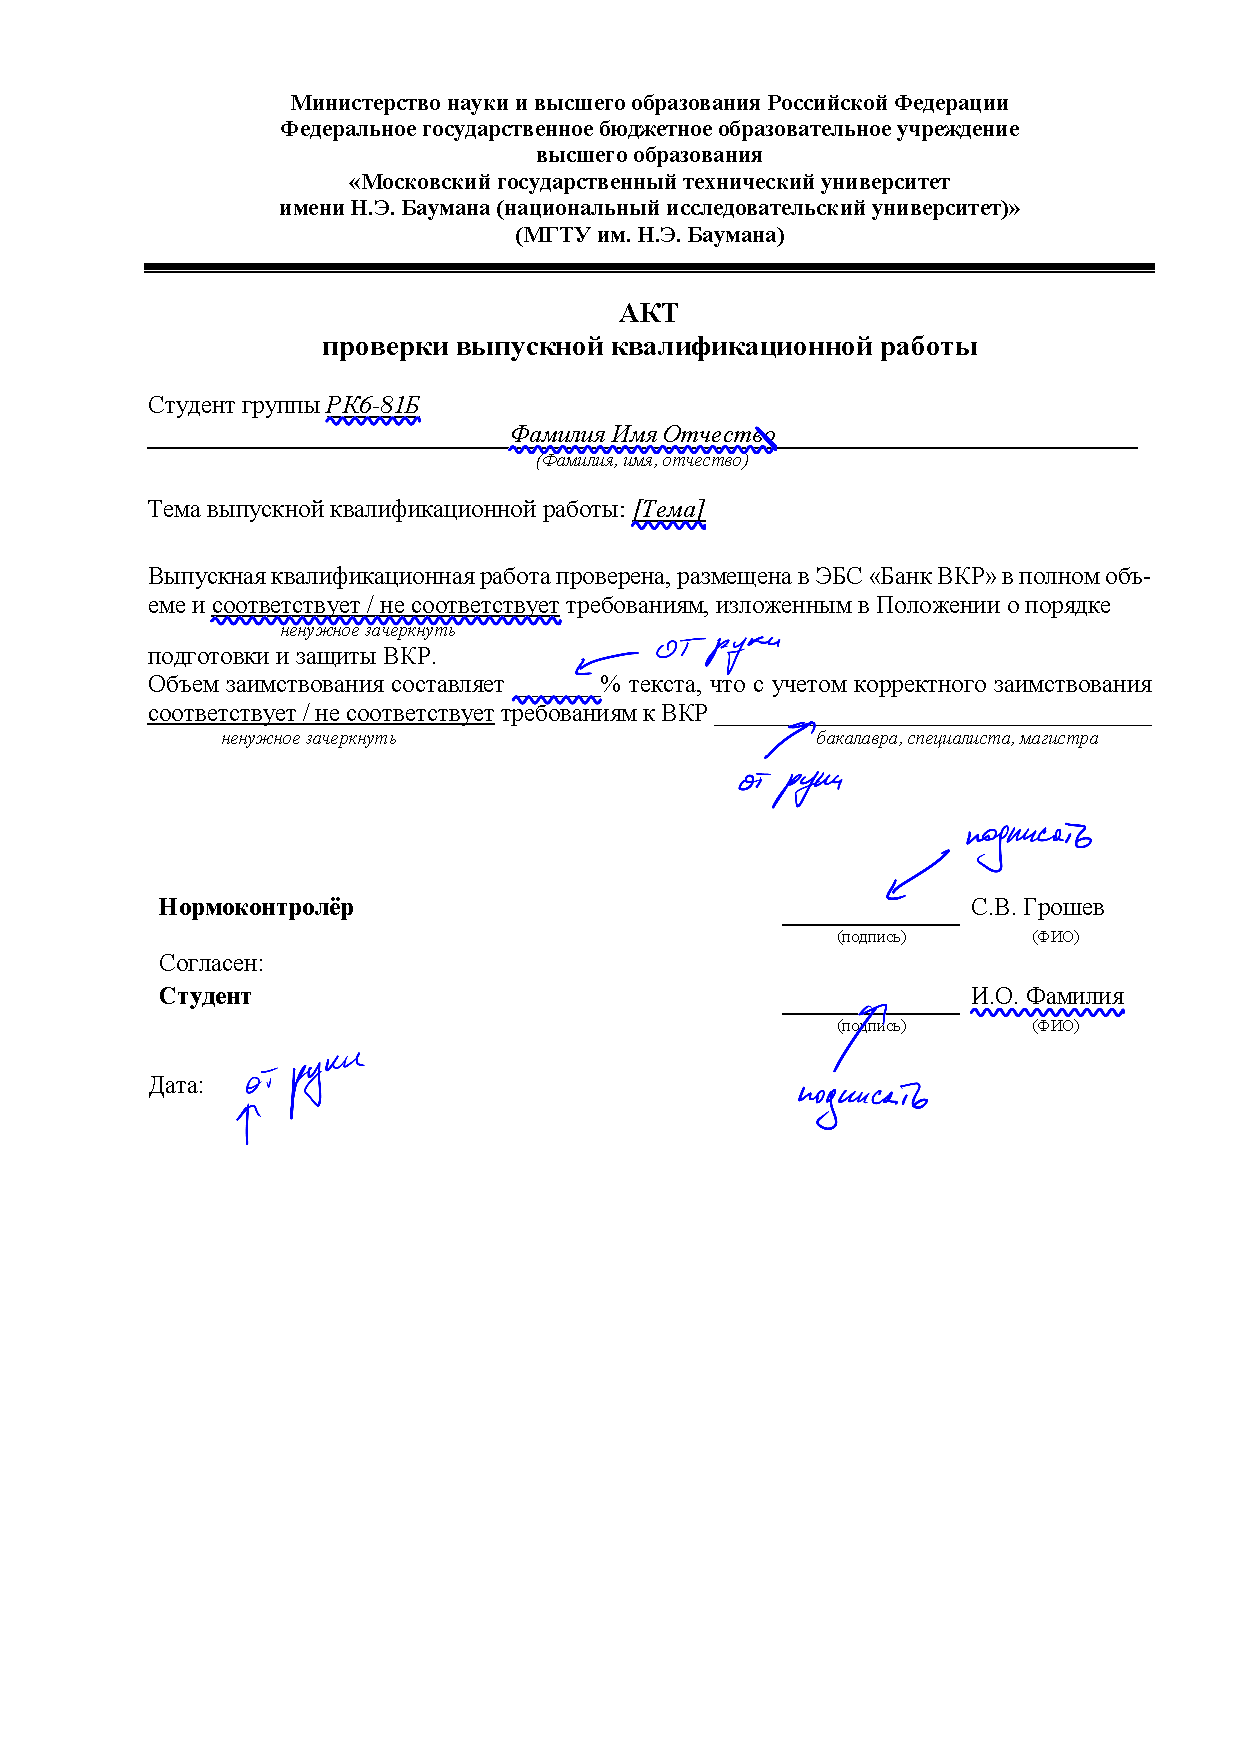
\includepdf{doc-additional/cpxsln_vkr_20YY_ShortTitle_group_SurnameNF_plagiarism.pdf}
}
%----------------------------------------------------------------

} 
%----------------------------------------------------------
%%приложения
%
% листы A1
% Акт об отсутствии заимствований
% Рецензии
%

\appendix

% команды далее необходимы для того, чтобы нумерация элементов текста в приложениях была корректной.
\renewcommand{\theequation}{\thechapter.\arabic{equation}}
\renewcommand{\thefigure}{\thechapter.\arabic{figure}}
\renewcommand{\thetable}{\thechapter.\arabic{table}}
% -------
\renewcommand{\appendixname}{ПРИЛОЖЕНИЯ}
\def\chaptername{ПРИЛОЖЕНИЕ}
\def\thechapter{\Asbuk{chapter}\unskip}
\renewcommand{\thesection}{\thechapter.\arabic{section}\unskip}
%%%%%%%%%%%%%%%%%%%%%%%%%%%%%%%%%%%%%%%%%%%%%%%%%%%%%%%%%%%%%%%%%%%%%%%%
\addcontentsline{toc}{chapter}{ПРИЛОЖЕНИЯ}
%%%%%%%%%%%%%%%%%%%%%%%%%%%%%%%%%%%%%%%%%%%%%%%%%%%%%%%%%%%%%%%%%%%%%%%%
% ПРИЛОЖЕНИЕ
\fancyhead[C]{\thepage \\ \textbf{\leftmark}}
\fancyfoot[C]{}
%----------------------------------------------------------------
\includepdfset{turn=true,scale=0.85,linktodoc=true,pages=-,pagecommand={\pagestyle{fancy}}}
%----------------------------------------------------------------
\chapter{}\label{apx_a1}




%{\catcode`\_=11
%\newpage
%\includepdf[pagecommand=\label{appx_A1_list1},pages=-]{appendices/appx_A1_list1.pdf}
%}
%
%%{\catcode`\_=11
%%\newpage
%%\includepdf[pagecommand=\label{appx_A1_list1},pages=-]{appendices/appx_A1_list1.pdf}
%%}
%%----------------------------------------------------------------
%\chapter{Акты и рецензии}\label{apx_acts_reviews}
%
%{\catcode`\_=11
%\newpage
%\includepdf[pagecommand=\label{appx_act_plagiat},pages=-]{appendices/appx_act_plagiatpdf}
%}
%
%{\catcode`\_=11
%\newpage
%\includepdf[pagecommand=\label{appx_review_1},pages=-]{appendices/appx_review_1.pdf}
%}

%%%%%%%%%%%%%%%%%%%%%%%%%%%%%%%%%%%%%%%%%%%%%%%%%%%%%%%%%%%%%%%%%%%%%%%%




%----------------------------------------------------------
% метка нужна для отслеживания общего числа страниц в документе
\label{lastpage}
%----------------------------------------------------------
\end{document}
%==========================================================



